\documentclass[a4paper,10pt,twoside]{article}
\usepackage[utf8x]{inputenc}
\usepackage[english]{babel} 
\usepackage[usenames,dvipsnames,figures]{xcolor}
\usepackage{lmodern,tikz,makeidx,graphicx,eurosym,amsmath,comment,titlesec,subcaption,textgreek,multirow,hyperref,url,enumerate,chemfig,sectsty,mathrsfs,amssymb,amsthm,multicol,fancyhdr,setspace,indentfirst,multicol,gensymb,textcomp,booktabs,bookmark,array,tikz,mathtools,tabulary}
\usepackage[neverdecrease]{paralist}
\usepackage[authoryear]{natbib}
\usepackage[autostyle]{csquotes}  
\usepackage[final]{pdfpages}
\usepackage{mhchem}
\usepackage[top=3cm, bottom=3cm, left=3cm, right=3cm]{geometry}
\usepackage[linesnumbered,ruled]{algorithm2e}
\usetikzlibrary{matrix,chains,positioning,decorations.pathreplacing,arrows}

\newtheorem{theorem}{Theorem}
\newcommand\myeq{\mathrel{\overset{\makebox[0pt]{\mbox{\normalfont\tiny\sffamily a}}}{=}}}

\RequirePackage{amsmath,amssymb,latexsym}
\hypersetup{
    colorlinks=false,       % false: boxed links; true: colored links
    linkcolor=black,          % color of internal links (change box color with linkbordercolor)
    citecolor=black,        % color of links to bibliography
    filecolor=black,      % color of file links
    urlcolor=black           % color of external links
}

\setlength\columnsep{26pt}

\newcommand\norm[1]{\left\lVert#1\right\rVert}

\newcommand\MyBox[2]{
  \fbox{\lower0.75cm
    \vbox to 1.7cm{\vfil
      \hbox to 1.7cm{\hfil\parbox{1.4cm}{#1\\#2}\hfil}
      \vfil}%
  }%
}

\newcommand{\HRule}{\rule{\linewidth}{0.5mm}} 
\newcommand{\angstrom}{\mbox{\normalfont\AA}}
\newlength{\drop}
\newtheorem{definition}{Definition}[section]

% Set TOC depth to only show sections.
\setcounter{tocdepth}{1}

\pagestyle{fancy}
\setlength{\headheight}{25pt} 
\lhead{\textbf{Philip Hartout}}
\rhead{\textbf{Introduction to Machine Learning - Summary}}
\rfoot{}

\title{Introduction to Machine Learning \\ Summary}
\author{Philip Hartout}
\date{\today}   

\begin{document}

\maketitle

\tableofcontents

\section{Linear Regression}
Objective, approximate:
\begin{align*}
    f(x) &= w_1x_1+\ldots+w_dx_d+w_0\\
        &= \sum_{i=1}^{d}w_ix_i+w_0\\
        &= \mathbf{w}^{T}\mathbf{x}+w_0
\end{align*}
$\forall \mathbf{x}, \mathbf{w}\in\mathbb{R}^{d}$. This expression can be further compressed to the homogeneous representation where $\forall \mathbf{\tilde{x}}, \mathbf{\tilde{w}}\in\mathbb{R}^{d+1}$, i.e. $\tilde{x}_{d+1}=1$. We have w.l.o.g.:
\begin{align*}
f(x) = \mathbf{w}^{T}\mathbf{x}
\end{align*}
Quantify errors using residuals:
\begin{align*}
    r_i &= y_i-f(x_i)\\
        &= y_i-\mathbf{w}^{T}\mathbf{x_i}
\end{align*}
We can use squared residuals and sum over all residuals to get the cost:
\begin{align}
    \label{objective_lse}
    \hat{R}(w) &= \sum_{i=1}^{n}r_i^2\\
               &= \sum_{i=1}^{n}(y_i-\mathbf{w}^{T}\mathbf{x_i})^2
\end{align}
Optimization objective to find optimal weight vector $\mathbf{w}$ with least squares is the following:
\begin{equation*}
    \mathbf{w} = \arg\min_{\mathbf{w}}\displaystyle\sum_{i=1}^{n}\left(y_i-w^{T}x_i\right)^2
\end{equation*}

\subsection{Closed form solution}
This can be solved in closed form:
\begin{equation*}
    \mathbf{\hat{w}} = (\mathbf{X}^{T}\mathbf{X})^{-1}\mathbf{X}^{T}\mathbf{y}
\end{equation*}

where:
\begin{equation*}
    X = 
    \begin{bmatrix}
        X_{1,1} & \ldots & X_{1,d}\\
        \vdots & \ddots & \vdots\\
        X_{n,1} & \ldots & X_{n,d}\\
    \end{bmatrix}        
    \text{ and }
    y = 
    \begin{bmatrix}
        y_{1} \\
        \vdots \\
        y_{n}
    \end{bmatrix}
\end{equation*}

\subsection{Optimization}
\subsubsection{Requirements}
Requires a convex objective function.
\begin{definition}[Convexity]
    A function is convex iff $\forall \mathbf{x},\mathbf{x}', \lambda\in[0,1] \text{ it holds that } f(\lambda x+(1-\lambda)x')\leq \lambda f(x)+(1-\lambda)f(x')$
\end{definition}
Note that the least squares objective function defined in \ref{objective_lse} is convex. 
\subsubsection{Gradient descent}
We start with an arbitrary $w_0\in\mathbb{R}^d$, then for $t=0,1,2,\ldots$ we perform the following operation:
\begin{equation*}
    w_{t+1} = w_t -\eta_t\nabla\hat{R}(w_t)
\end{equation*}
where $\eta_t$ is the learning rate.\\
Under mild assumptions, if the step size is sufficiently small, the gradient descent procedure converges to a stationary point, where the gradient is zero. For convex objectives, it therefore finds the optimal solution. In the case of the squared loss and a constant step size (e.g. 0.5), the algorithm converges at linear rate. If you look at the difference in empirical value at iteration $t$ and compare that with the optimal value, then the gap is going to shrink at linear rate. If we look for a solution within a margin $\epsilon$, it is found in $\mathcal{O}(\ln(\frac{1}{\epsilon}))$ iterations.  The fact that the objective function congerges at linear rate can be formally described 
as follows:

\begin{equation*}
    \exists t_0 \forall t\geq t_0, \exists \alpha<1 \text{ s.t. } (\hat{R}(w_{t+1})-\hat{R}(\hat{w}))\leq\alpha(\hat{R}(w_{t})-\hat{R}(\hat{w}))
\end{equation*}

where $\hat{w}$ is the optimal value for the hyperparameters.\\
For computing the gradient, we recall that:
\begin{equation*}
    \nabla\hat{R}(\hat{w}) = 
    \begin{bmatrix}
        \frac{\partial}{\partial w_1}\hat{R}(w) & \ldots & \frac{\partial}{\partial w_d}\hat{R}(w)
    \end{bmatrix}
\end{equation*}
In one dimension, we have that:
\begin{align*}
    \nabla\hat{R}(w) &= \frac{d}{dw}\hat{R}(w) = \frac{d}{dw}\sum_{i=1}^{n}(y_i-w\cdot x_i)^2\\
    &= \sum_{i=1}^{n}\frac{d}{dw}(y_i-w\cdot x_i)^2\\
    &=2(y_i-w\cdot x_i)\cdot(-x_i)\\
    &=\sum_{i=1}^{n}2(y_i-w\cdot x_i)\cdot(-x_i)\\
    &=-2\sum_{i=1}^{n}r_i x_i.\\
\end{align*}
In $d$-dimension, we have that:
\begin{equation*}
    \nabla\hat{R}(w)=-2\sum_{i=1}^{n}r_i x_i,
\end{equation*}
where $r_i\in\mathbb{R}$ and $x_i\in\mathbb{R}^d$

\subsubsection{Adaptive step size for gradient descent}

The step size can be updates adaptively, via either:
\begin{enumerate}
    \item \textbf{Line search}:\\
    Suppose at iteration $t$, we have $w_t$, $g_t=\nabla\hat{R}(w_t)$. We then define:
    \begin{equation*}
        y_t^{*} = \arg\min_{y\in[0,\infty)}\hat{R}(w_t)-\eta g_t
    \end{equation*}
    \item \textbf{Bold driver heuristic}:
    \begin{itemize}
        \item If the function decreases, increase the step size.
        \begin{equation*}
            \text{If }\hat{R}(w_{t+1})<\hat{R}(w_{t}): \eta_{t+1}\leftarrow\eta_{t}\cdot c_{acc}
        \end{equation*}
        where $c_{acc}>1$
        \item If the function increases, decrease the step size. 
        \begin{equation*}
            \text{If }\hat{R}(w_{t+1})>\hat{R}(w_{t}): \eta_{t+1}\leftarrow\eta_{t}\cdot c_{dec}
        \end{equation*}
        where $c_{dec}<1$.
    \end{itemize}
\end{enumerate}
\subsubsection{Tradeoff between gradient descent and closed form}
Several reasons:
\begin{itemize}
    \item Computational complexity:
    \begin{equation*}
        \hat{w}=(X^TX)^{-1}(X^Ty)
    \end{equation*}
    $(X^TX)$ can be computed in $\mathcal{O}(nd^2)$, $(X^TX)^{-1}$ can be computed in $\mathcal{O}(d^3)$.\\
    By comparison, for gradient descent calculating $\nabla\hat{R}(w)=\sum_{i=1}^{n}(y_i-w^Tx_i)x_i$ can be computed in $\mathcal{O}(nd)$, where $n=\ln(\frac{1}{\epsilon})$
    \item the problem may not require an optimal solution.
    \item many problems do not admit a closed form solution.
\end{itemize}
\subsection{other loss functions}
Least squares is part of a general case of the following general loss function, which is convex for $p\geq 1$.
\begin{equation}
    l_p(r)=|r|^p
\end{equation}
Least squares is where $p=2$.

\section{Probability (interlude)}
\subsection{Gaussians}

The p.d.f. of a Gaussian distribution is given by:
\begin{equation}
    \frac{1}{\sqrt{2\pi\sigma^2}}\exp\left(-\frac{x-\mu}{2\sigma^2}\right)
\end{equation}
The p.d.f. of a multivariate Gaussian distribution is given by:
\begin{equation}
    \frac{1}{2\pi\sqrt{|\sigma|}}\exp\left(-\frac{1}{2}(x-\mu)^T\sigma^{-1}(x-\mu)\right)
\end{equation}
where:
\begin{equation}
    \sigma = \begin{pmatrix}
        \sigma_{1}^2, \sigma_{12}\\
        \sigma_{21}, \sigma_{2}^2
    \end{pmatrix}
    \text{ and }
    \begin{pmatrix}
        \mu_1\\
        \mu_2
    \end{pmatrix}
\end{equation}
\subsection{Expectations}
Expected value of a random variable can be calculated as follows:
\begin{equation*}
    \mathbb{E}=\begin{cases}
        \sum_{x}xp(x)\qquad\text{if }X\text{ is discrete}\\
        \int xp(x)dx\qquad\text{if }X\text{ is continuous}\\
    \end{cases}
\end{equation*}
Expectations respect linear properties, i.e. let $X, Y$ be random variable and 
$a,b\in\mathbb{R}$, then we have $\mathbb{E}[aX+bY]=a\mathbb{E}[X]+b\mathbb{E}[Y]$.

\section{Generalization and model validation}

\subsection{Fitting nonlinear functions via linear regression}

Using nonlinear features of our data (basis functions), we can fit nonlinear functions via linear regression. Then, the model takes on the form:

\begin{equation}
    f(\mathbf{x}) = \sum_{i=1}^{d}w_i\phi(\mathbf{x})
\end{equation}

where $\mathbf{x}\in\mathbb{R}^d$, $x\mapsto \tilde{x}=\phi(\mathbf{x})\in\mathbb{R}^d$ and $w\in\mathbb{R}^d$. 
\begin{itemize}
    \item 1 dim.: $\phi(\mathbf{x})=\begin{bmatrix}
        1,x, x^2, \ldots, x^k
    \end{bmatrix}$
    \item 2 dim.: $\phi(\mathbf{x})=\begin{bmatrix}
        1,x_1, x_2, x_1^2, x_2^2, \ldots, x_1^k, x_2^k
    \end{bmatrix}$
    \item p dim.: $\phi(\mathbf{x})$ vector of all monomials in $x_1,\ldots, x_p$ of degree up to $k$.
\end{itemize}

\subsection{Achieving generalization}
\subsubsection{Independence and identical distribution}
A fundamental assumption needs to be met: the dataset is generated from an independently and identically distributed from some unknown distribution $P$, i.e:
\begin{equation*}
    (x_i, y_i)\sim P(\mathbf{X},Y).
\end{equation*}

The i.i.d. assumption is invalid when:
\begin{itemize}
    \item we deal with time series data
    \item spatially correlated data
    \item correlated noise
\end{itemize}
If violated, we can still use ML but the interpretation of the results needs to be carefully analyzed. The most important thing is to choose the train/test split to assess the desired generalization properties of the trained model. 

\subsection{Expected error and generalization error}
Once the iid assumption is verified, our goal is then to minimize the expected error (true risk) under $P$, i.e.:
\begin{align*}
    R(\mathbf{w})&=\int P(\mathbf{x},y)(y-\mathbf{w}^T\mathbf{x})^2dxdy\\
    & =\mathbb{E}[(y-\mathbf{w}^T\mathbf{x})^2]
\end{align*}
The true risk can be estimated by the empirical risk on a sample dataset $D$:
\begin{equation*}
    \hat{R}_D(\mathbf{w})=\frac{1}{|D|}\sum_{\mathbf{x}, y\in D}(y-\mathbf{w}^T\mathbf{x})^2
\end{equation*}
The reason behind this approximation is because of the law of large numbers
\begin{definition}[Law of large numbers]
    $\hat{R}_D(\mathbf{w})\rightarrow R_D(\mathbf{w})$ for any fixed $\mathbf{w}$ as $|D|\rightarrow\infty$.
\end{definition}
\begin{equation}
    \label{empirical_risk}
    \mathbf{\hat{w}}_D=\arg\min_{\mathbf{w}}\hat{R}_D(\mathbf{w})
\end{equation}

\begin{equation}
    \label{true_risk}
    \mathbf{w*}=\arg\min_{\mathbf{w}}\hat{R}(\mathbf{w})
\end{equation}

We don't want to minimize the empirical risk given in equation \ref{empirical_risk} but the true risk given in equation \ref{true_risk}, which are similar as the amount points in the dataset increases.

\subsection{Uniform convergence}

For learning via empirical risk minimization, uniform convergence is required, i.e.:
\begin{equation*}
    \sup_{\mathbf{w}}|R(\mathbf{w})-\hat{R}_D(\mathbf{w})|\rightarrow 0 \text{ as }|D|\rightarrow\infty
\end{equation*}

Note that this is not implied by the law of large numbers alone, but depends on model class. It holds for instance for squared loss on data distributions with bouded support. Statistical learning theory is required to define these properties.

\subsection{Evaluation of performance on training data}

In general in holds that:
\begin{equation*}
    \mathbb{E}_D[\hat{R}_D(\hat{\mathbf{w}}_D)]\leq\mathbb{E}_D[R_D(\hat{\mathbf{w}}_D)]
\end{equation*}
\begin{proof}[Proof]
    \begin{align*}
        \mathbb{E}[\hat{R}_D(\hat{\mathbf{w}}_D)] &= \mathbb{E}_D[\min_{\mathbf{w}}\hat{R}_D(\mathbf{w})]\qquad\text{(ERM)}\\
        &\leq \min_{\mathbf{w}}\mathbb{E}_D[\hat{R}_D(\mathbf{w})]\qquad\text{(Jensen's inequality)}\\
        &= \min_{\mathbf{w}}\mathbb{E}_D[\frac{1}{|D|}\sum_{i=1}^{|D|}(y_i-wx_i)^2]\qquad\text{(Definition of $\hat{R}_D(.)$)}\\
        &= \min_{\mathbf{w}}\mathbb{E}_D[\frac{1}{|D|}\sum_{i=1}^{|D|}(y_i-wx_i)^2]\qquad\text{(linear expectations)}\\
        &= \min_{\mathbf{w}}R(\mathbf{w})\leq\mathbb{E}[R(\hat{w}_D)]\\
    \end{align*}
\end{proof}
Thus, we obtain an overly optimistic estimate. A more realistic evaluation would be to use a separate test set from the same distribution $P$. Then:
\begin{itemize}
    \item Optimize $w$ on training set:
    \begin{equation*}
        \mathbf{\hat{w}}_{D_{\text{train}}} = \arg\min_{\mathbb{w}} \hat{R}_{\text{train}}(\mathbb{w})
    \end{equation*}
    \item Evaluate on test set:
    \begin{equation*}
        \hat{R}_{\text{test}}(\mathbf{\hat{w}})=\frac{1}{|D_{\text{test}}|}\sum_{\mathbf{x},y\in D_{\text{test}}}^{}(y-\hat{\mathbf{w}}^T\mathbf{x})^2
    \end{equation*}
    \item Then:
    \begin{equation*}
        \mathbb{E}_{D_{\text{train}}, D_{\text{test}}}[\hat{R}_{D_{\text{test}}}(\hat{\mathbf{w}}_{D_{\text{train}}})]=\mathbb{E}_{D_{\text{train}}}[R(\mathbf{\hat{w}}_{D_{\text{train}}})]
    \end{equation*}
\end{itemize}
\begin{proof}[Proof]
    Let $D_train=D$, $D_test=V$ and $D,V\sim P$. Then:
    \begin{align*}
        \mathbb{E}_{D,V}[\hat{R}_V(\hat{\mathbf{w}}_D)] &= \mathbb{E}_D[\mathbb{E}_V[\hat{R}_V(\hat{\mathbf{w}}_D)]]\qquad\text{independence of $D,V$}\\
        &=\mathbb{E}_D[\mathbb{E}_V[\frac{1}{|V|}\sum_{i=1}^{|V|}(y_i-\hat{\mathbf{w}}_D^Tx_i)^2]]\qquad\text{(Definition of $\hat{R}_D(.)$)}\\
        &=\mathbb{E}_D[\frac{1}{|V|}\sum_{i=1}^{|V|}\mathbb{E}_{x_i, y_i}(y_i-\hat{\mathbf{w}}_D^Tx_i)^2]\qquad\text{since $(x_i,y_i)\bot D$}\\
        &=\mathbb{E}_D[R(\mathbf{\hat{w}}_D)]   
    \end{align*}
\end{proof}
\subsection{Evaluation for model selection}
For each candidate model $m$, we repeat the following procedure for $i=1:k$:
\begin{itemize}
    \item We split the same dataset into training and validation sets:
    \begin{equation*}
        D=D_{\text{train}}^{(i)}\biguplus D_{\text{val}}^{(i)}
    \end{equation*}
    \item We train the model:
    \begin{equation*}
        \hat{\mathbb{w}}_[i,m]=\arg\min_{\mathbf{w}}\hat{R}_{\text{train}}^{(i)}(\mathbf{w})
    \end{equation*}
    \item Then we estimate the error:
    \begin{equation*}
        \hat{R}_{m}^{(i)}=\hat{R}_{\text{val}}^{(i)}(\hat{\mathbf{w}}_i)
    \end{equation*}
\end{itemize}
Finally, select the model:
\begin{equation*}
    \hat{m}=\arg\min_{m}\frac{1}{k}\sum_{i=1}^{k}\hat{R}_{m}^{(i)}
\end{equation*}
\subsection{Splitting the data for model selection}
This splitting can be done randomly through Monte Carlo cross-validation. 
\begin{itemize}
    \item Pick training set of given size uniformly at random
    \item Validate on remaining points
    \item Estimate prediction error by averaging the validation error over multiple random trials.
\end{itemize}
It can also be achieved through $k$-fold cross-validation, which is the default choice.
\begin{itemize}
    \item Partition the data into $k$ folds
    \item Train on $k-1$ folds, evaluating on remaining fold.
    \item Estimate prediction error by averaging the validation error obtained while varying the validation fold.
\end{itemize}
Note that the cross-validation error is almost unbiased for large enough $k$. The following should be considered to pick $k$:
\begin{itemize}
    \item Too small: 
    \begin{itemize}
        \item Risk of overfitting on test set
        \item Using too little data for training
        \item Risk of underfitting to training set
    \end{itemize}
    \item Too large:
    \begin{itemize}
        \item In general, leads to better performance. $k=n$ is perfectly fine, specific instance called leave-one-out cross-validation
        \item Higher computational complexity.
    \end{itemize}
\end{itemize} 
In practice, $k=5$ or $k=10$ is ofen used and works well.
\subsection{Best practice for evaludating models in supervised learning}
Follow the following steps:
\begin{itemize}
    \item Split data set into training and test set
    \item Never look at test set when fitting the model. For example, use $k$-fold cross-validation on training set
    \item Report final accuracy on test set, but never optimize on it.
\end{itemize}
Note that this procedure only works if the data is i.i.d. I.e. one should be careful if there are temporal trends or other dependencies.

\section{Regularization}
We want to avoid having overly complex models when minimizing the loss function. This can be achieved through regularization, which encourages small weights via penalty functions, which are called regularizers.

\subsection{Ridge regression}
This is a regularized optimization problem:
\begin{equation*}
    \min_{\mathbf{w}}\frac{1}{n}\sum_{i=1}^{n}(y_i-\mathbf{w}^Tx_i)^2+\lambda\norm{\mathbf{w}}^{2}_{2}=\sum_{j=1}^{d}\mathbf{w}_j^2\qquad\forall\lambda\geq 0
\end{equation*}
\subsubsection{Closed form solution}
This can be optimized using the closed form solution or gradient descent. The closed form for Ridge regression is:
\begin{equation*}
    \mathbf{\hat{w}}=(\mathbf{X}^T\mathbf{X}+\lambda\mathbf{R})^{-1}\mathbf{X}^Ty
\end{equation*}
where $I\in\mathbb{R}^{d\times d}$ is the identity matrix.
\subsubsection{Gradient descent}
\begin{equation*}
    \nabla\left(\frac{1}{n}\sum_{i=1}^{n}(y_i-\mathbf{w}^T\mathbf{x}_i)^2 + \lambda\norm{\mathbf{w}}^{2}_{2}\right) = \nabla_{\mathbf{w}}\hat{R}(\mathbf{w})+\lambda \nabla_{\mathbf{w}}\norm{\mathbf{w}}^{2}_{2}
\end{equation*}
One step of the gradient descent is therefore performed as follows:
\begin{align*}
    w_{t+1}&\leftarrow w_t-\eta_t(\nabla_{\mathbf{w}}\hat{R}(\mathbf{w}_t)+2\lambda\mathbf{w}_t)\\
    &=(1-2\lambda\eta_t)\mathbf{w}_t-\eta_t\nabla_{\mathbf{w}}\hat{R}(\mathbf{w}_t)
\end{align*}
Choosing the regularization parameter is done through cross-validation. Typically, the choice is between values of $\lambda$ values which are logarithmically spaced.
\subsubsection{Generalization of a tradeoff in ML}
A lot of supervised learning problems can be written in this way:
\begin{equation*}
    \min_{\mathbf{w}}\hat{R}(\mathbf{w})+\lambda C(\mathbf{w}).
\end{equation*}
It's possible to control complexity by varying regulzation parameter $\lambda$. 
\subsection{Renormalizing data through standardization}
This process ensures that each feature has zero mean and unit variance:

\begin{equation*}
    \tilde{x}_{i,j}=\frac{(x_{i,j})-\hat{\mu}_{j}}{\hat{\sigma}}_j
\end{equation*}

where $x_{i,j}$ is the value of the $j$\textsuperscript{th} feature of the $i$\textsuperscript{th} data point:

\begin{equation*}
    \hat{\mu}_j=\frac{1}{n}\sum_{i=1}^{n}x_{i,j} \qquad \sigma_j^2 = \frac{1}{n}\sum_{i=1}^{n}(x_{i,j}-\hat{\mu}_j)^2
\end{equation*}

\section{Classification}
\begin{definition}[Classification]
    Classification is an instance of supervised learning where $Y$ is discrete (categorical). We wanto to assign data points $X$ (documents, queries, images, user visits) a label $Y$ (spam/not spam, topic such as sports, politics, entertainment, click/no-click etc).
\end{definition}

The input of the model is labeled data set with positive and negative examples, see Figure \ref{binary_classification}. The output is a decision rule, i.e. a hypothesis.
\begin{figure}[htbp]
    \centering
    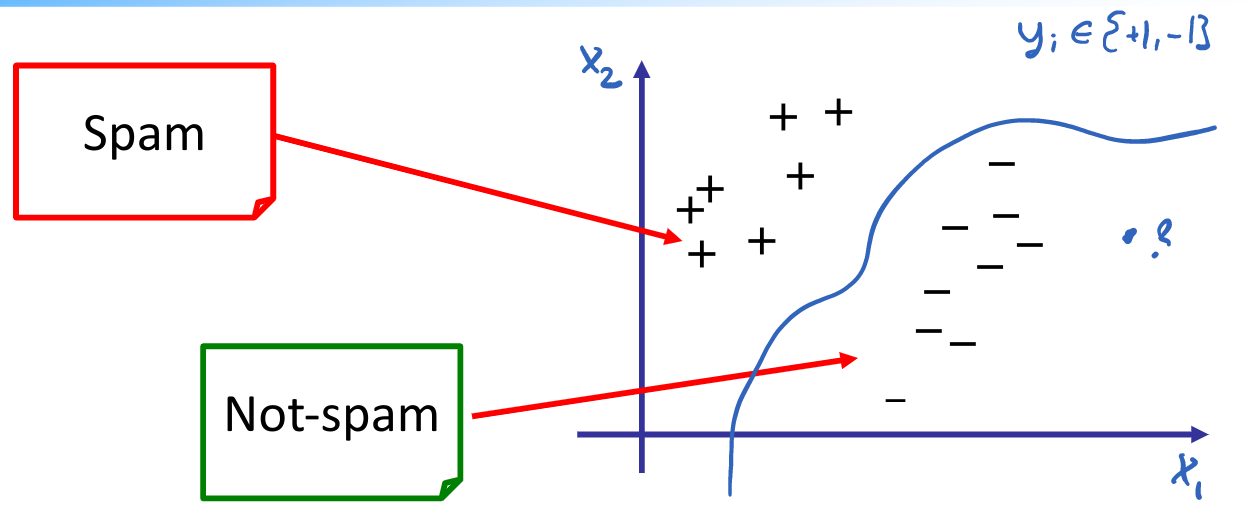
\includegraphics[width=.5\textwidth]{figures/binary_classification.png}
    \caption{Illustration of binary classification}
    \label{binary_classification}
\end{figure}
Given a dataset $D=\left\{(x_1, y_1), \ldots(x_n, y_n)\right\}$, we have:
\begin{equation*}
    y\approx h_{\mathbf{w}}(x)= \text{sign}(w^Tx)
\end{equation*}
Linear classification works well in high-dimensional settings when using the right features; prediction is typically very efficient despite linear classification seeming very restrictive at first.

\subsection{Finding linear separators}

Writing the search for a classifier can be seen as an optimization problem:
we seek the set of weights $\mathbf{w}$ that minimizes the number of mistakes, i.e.:
\begin{align*}
    \hat{\mathbf{w}} &= \arg\min_{\mathbf{w}\in\mathbb{R}}\sum_{i=1}^{n}[y_i\neq \text{sign}(w^Tx_i)]\\
    =\begin{cases}
        1\text{ if } y_i\neq \text{sign}(w^Tx_i)\\
        0\text{ otherwise.}
    \end{cases}
\end{align*}

The goal is then to optimize the following function:
\begin{align*}
    \hat{\mathbf{w}} &= \arg\min_{\mathbf{w}\in\mathbb{R}}\frac{1}{n}\sum_{i=1}^{n}[y_i\neq \text{sign}(w^Tx_i)]\\
    &= \frac{1}{n}\sum_{i=1}^{n}\mathcal{l}(w; x_i,y_i)
\end{align*}
Note that this poses as challenge as it is not convex or even differentiable. Therefore we need to replace this loss by a tractable loss function for the sake of optimization/model fitting. When evaluating a model, we then use the original cost/performance function. The function we can use to optimize in this case is the surrogate loss:
\begin{equation*}
    l_P(\mathbf{w}; y_i, x_i) = \max (0, -y_i\mathbf{w}^Tx_i)
\end{equation*}
which is also referred to as the perceptron loss.

The gradient of the perceptron loss function can be computed as follows:
\begin{align*}
    \hat{R(w)}&=\sum_{i=1}^{n}\max (0, -y_iw^Tx_i)\\
    \nabla\hat{R(w)}&=\sum_{i=1}^{n}\nabla_{\mathbf{w}}\max (0, -y_iw^Tx_i)\\
    &=\begin{cases}
        0\text{ if } y_iw^Tx_i\geq 0 \text{ i.e. correctly classified }
        -y_ix_i\text{ otherwise} 
    \end{cases}
\end{align*}

So we have the following update rule:
\begin{equation*}
    \mathbf{w}_{t+1} \leftarrow \mathbf{w}w_t+\eta_t\sum_{i:(x_i,y_i) {incorrectly classified by} w}^{x_iy_i}
\end{equation*}

\subsection{Stochastic gradient descent}
Computing the gradient requires summing over all data, which is inefficient for large datasets. Additionally, our initial estimates are likely very wrong and we can get a good unbiased gradient estimate by evaluating the gradient on few points. In the worst case, we can evaluate only one randomly chosen point, which is a procedure called stochastic gradient descent. It consists of the following steps:
\begin{enumerate}
    \item Start at an arbitrary $\mathbf{w}_0\in\mathbb{R}^d$
    \item For $t=1,2,\ldots$ do:
    \begin{itemize}
        \item Pick data point $(\mathbf{x}',y')\in D$ from training set uniformly at random (with replacement), and set:
        \begin{equation*}
            \mathbf{w}_{t+1}=\mathbf{w}_t-\eta_t\nabla\mathcal{l}(\mathbf{w}_t;\mathbf{x}',y')
        \end{equation*}
    \end{itemize}
\end{enumerate}
Where $\eta_t$ is called the learning rate. Guaranteed to converge under mild conditions, if:
\begin{equation*}
    \sum_{t}\eta_t=\infty \text{ and }\sum_{t}\eta_t^2<\infty
\end{equation*}
for instance $\eta_t=\frac{1}{t}$ and $\eta_t=\min (c, \frac{c'}{t})$.\\
The perceptron algorithm is just stochastic gradient descent on the perceptron loss function $\mathcal{l}_P$ with learning rate 1.
\begin{theorem}[Perceptron algorithm]
    If the data is linearly separable, the perceptron will obtain a linear separator.
\end{theorem}
The variance of the gradient estimate can be reduced by averaging over the gradients w.r.t. multiple randomly selected points, which are called minibatches. Adaptive learning rates can be additionally applie. There exist various approaches for adaptively tuning the learning rate. Often times, these even use a different learning rate per feature. Examples of adaptive learning rate algorithms include AdaGrad, RMSProp, Adam, ...
\subsection{Hinge loss vs. perceptron loss}
The Hinge loss encourages the margin of the classifier, and is defined as follows:
\begin{equation*}
    \mathcal{l}_H(\mathbf{w}; \mathbf{x}, y)=\max\left\{0,1-y\mathbf{w}^T\mathbf{x}\right\}
\end{equation*}

\subsection{Support vector machines}

The optimization objective for the support vector machine is defined as minimizing Hinge loss while also adding another regularization term. There are several lines that need to be considered in the max. margin linear classification, which are summarised in figure \ref{planes_svm}

\begin{figure}
    \centering
    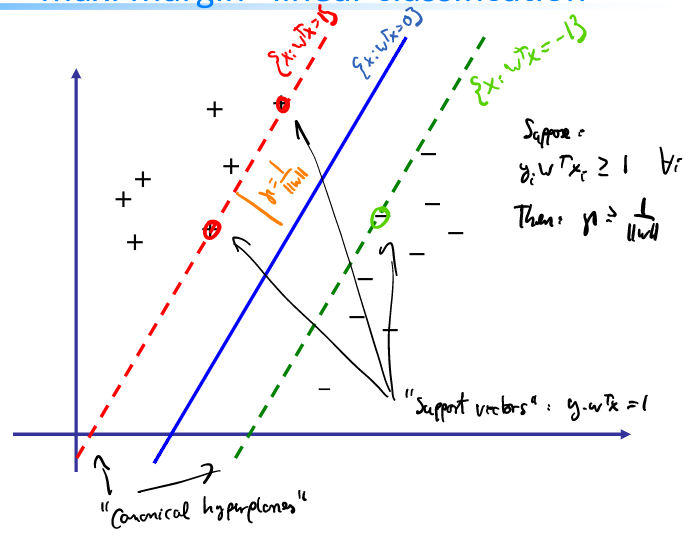
\includegraphics[width=.8\textwidth]{figures/max_margin_decision_boundaries.png}
    \caption{Important elements and their defining equations for support vector machines.}
    \label{planes_svm}
\end{figure}

Support vector machinea re widely used, very effective linear classifiers. They behave almost like a perceptron. The only differences include:
\begin{itemize}
    \item Optimize slightly different, shifted loss (hinge loss)
    \item They regularize the weights
\end{itemize}
It can be optimized using a stochastic gradient descent. A safe choice for the learning rate is:
\begin{equation*}
    \eta_t=\frac{1}{\lambda t}
\end{equation*}

\subsubsection{Stochastic gradient descent for support vector machines}

Let's recall the ojective function:
\begin{equation*}
    \hat{R}(\mathbf{w})=\sum_{i=1}^{n}\mathcal{l}_{H}(\mathbf{w}_i; x_i,y_i) + \lambda\norm[{\mathbf{w}}_2^2
\end{equation*}
This requires taking care of the regularizer, as follows:
\begin{equation*}
    \hat{R}(\mathbf{w})=\sum_{i=1}^{n}\left(\mathcal{l}_{H}(\mathbf{w}_i; x_i,y_i) + \frac{\lambda}{n}\norm[{\mathbf{w}}_2^2\right)=f_i(\mathbf{w})
\end{equation*}
So, in order to estimate the gradient $\nabla_{\mathbf{w}}\hat{R}(\mathbf{w})$ which is equivalent to:
\begin{equation*}
    \nabla_{\mathbf{w}}\hat{R}(\mathbf{w})=\sum_{i=1}^{n}\nabla_{\mathbf{w}}f_{i}(\mathbf{w})
\end{equation*}
where:
\begin{equation*}
    \nabla_{\mathbf{w}}f_{i}(\mathbf{w}) = \nabla\mathcal{l}_{H}(\mathbf{w}+\frac{\lambda}{n}\nabla\norm{\mathbf{w}}_2^2)
\end{equation*}
so the gradient of the regularization term is just $2\mathbf{w}$. For the Hinge loss:
\begin{equation*}
    \nabla\mathcal{l}_H = \nabla\max(0,1-y_i\mathbf{w}^Tx_i)
    = \begin{cases}
        0\text{ if } y_iw^Tx_i\geq 1\\
        -y_ix_i\text{ otherwise.}
    \end{cases}
\end{equation*}
Therefore the entire update rule for stochastic gradient descent for SVM is:
\begin{equation*}
    \mathbf{w}_{t+1}\leftarrow w_t\left(1-\eta_t\frac{2\lambda}{n}\right)+\left[y_iw^Tx_i\right]
\end{equation*}
The regularization parameter can be picked via cross-validation just like in linear regression. Instead of using the Hinge loss for validation, the target performance metric needs to be used.

\subsection{Key takeaways}
The key takeaways are:
\begin{itemize}
    \item The perceptron is an algorithm for linear classification
    \item It applies SGD on the perceptron loss
    \item Mini-batches exploit parallelism and reduce variance compared to a single sample
    \item The perceptron loss is a convex surrogate function for the 0-1 misclassification loss
    \item It is guaranteed to produce a feasible solution if the data is separable
    \item SGD is much more generally applicable
    \item SVMs are closely related to Perceptron, they use a hinge loss and regularization.
\end{itemize}
Summary so far:
\begin{itemize}
    \item List of represnetations/features: linear hypotheses, nonlinear hypotheses with nonlinear feature transforms.
    \item Model/Objective: loss function (squared loss, 0/1 loss, perceptron loss, Hinge loss) + regularization ($L^2$ norm)
    \item Method: exact solution, gradient descent, mini-batch SGD, convex programming.
    \item Evaluation metric: MSE, accuracy
    \item Model selection: k-fold cross-validation, Monte Carlo CV.
\end{itemize}

\section{Feature selection}
Reasons why we don't want to work with all potentially available features:
\begin{itemize}
    \item interpretability: understand which features are most important
    \item generalizationL simpler models may generalize better
    \item storage computation and cost: if we select the most important features we don't need to store, sum and acquire data for unused features. 
\end{itemize}
The naive way to select features is to try all subsets and pick the best features via cross-validation. Greedy feature selection, which is a general purpose approach, consists of greedily add or remove features to maximize cross-validated prediction accuracy and mutual information or other notions of informativeness not discussed here. It can be used for any method, not only linear regression or classifiers. 

\subsection{General greedy approach}
Consider the set of features $V=\left\{1,\ldots, d\right\}$. We then define the cost function for scoring subsets S of V. $\hat{L}(S)$ is the cross-validation error using features in S only. More precisely: 
\begin{equation*}
    \mathbf{x}_i=[x_{i,1},\ldots,x_{i,d}]\rightarrow\mathbf{x}_{S,i}=[x_{i,j},\ldots,x_{i,j_k}]
\end{equation*}
where $S$ is defined as:
\begin{equation*}
    S=\left\{j,\ldots,j_{k}\right\}, k=|k|
\end{equation*}
We then train the model on $\left\{x_{j,1},y_1,\ldots,x_{j,n},y_n\right\}$, in order to obtain an estimate based on the weights $\hat{\mathbf{w}}_S$ with associated loss $\hat{L}(S)$, which represents the cross-validated performance of the weight estimates $\hat{\mathbf{w}}_S$.

\subsection{Greedy forward selection}
Start with $S=\emptyset$ and $E_0=\infty$, then for $i=1:d$, we find the best element to add, i.e.:
\begin{equation*}
    s_i=\arg\min{j\in V \setminus S}\hat{L}()S\cup \left\{j\right\}
\end{equation*}
then we compute the error:
\begin{equation*}
    E_i=\hat{L}(S\cup\left\{s_i\right\})
\end{equation*}
if $E_i>E_{i-1}$ break, else set $S\leftarrow \cup\left\{s_i\right\}$

\subsection{Greedy backward selection}
Start with $S=V$ and $E_{d+1}=\infty$, then for $i=d:-1:1$, we find the best element to remove, i.e.:
\begin{equation*}
    s_i=\arg\min{j\in S}\hat{L}(S\setminus\left\{j\right\})
\end{equation*}
then we compute the error:
\begin{equation*}
    E_i=\hat{L}(S\setminus\left\{s_i\right\})
\end{equation*}
if $E_i>E_{i-1}$ break, else set $S\leftarrow \setminus\left\{s_i\right\}$

\subsection{Advantages and drawbacks of forward vs. backward feature selection}
\begin{table}[htbp]
    \centering
    \begin{tabular}{lll}
        \toprule
        & Forward Feature Selection & Backward Feature Selection\\
        \midrule
        Method Advantages & Faster (if few relevant features) & Can handle ``dependent'' features\\
        \midrule
        Method drawback & Computational cost & Computational cost \\
        \midrule
        & Suboptimal & Suboptimal \\
        \bottomrule
    \end{tabular}
\end{table}

We want a method that simultaneously solves the learning and the feature selection problem via a single optimization step. So far we have only done optimization via sparsity: i.e. explicitely select a subset of features. This is equivalent to constraining $\mathbf{w}$ to be sparse, i.e. contain at most $k$ non-zero entries. Alternatively, we can penalize the number of nonzero entries: 
\begin{equation*}
    \hat{\mathbf{w}} = \arg\min_{\mathbf{w}}\sum_{i=1}^{n}(y_i-w^Tx_i)^2+\lambda \norm{w}_0
\end{equation*}
However, this is a difficult combinatorial optimization problem. The key idea then is to replace $\norm{\mathbf{w}}_0$ by a more tractable term. 

The idea here is to use $L_1$ as a surrogate for $L_0$, where:
\begin{equation*}
    \norm{w}_1=\sum_{i=1}^{d}|w_i|
\end{equation*}
and we use $\norm{w}_1$ instead of $\norm{w}_0$.

\subsection{Lasso regression}

In ridge regression, we use $\norm{\mathbf{w}}_2^2$ to control the weights. In Lasso, we replace $\norm{\mathbf{w}}_2^2$ by $\norm{\mathbf{w}}_1$, hence leading to the following L1-regularized regression:
\begin{equation*}
    \min_{\mathbf{w}}\lambda\norm{w}_1+\sum_{i=1}^{n}(y_i-\mathbf{w}^Tx_i)^2
\end{equation*}
This alternative penalty encourages coefficients to be exactly 0, which entails an automatic feature selection.

The regularization parameter can be picked using cross-validation.

\subsubsection{L1 regularization in SVM}
The sparsity trick can be applied to SVMs as well:
\begin{equation*}
    \min_{\mathbf{w}}\norm{\mathbf{w}}_1+\sum_{i=1}^{n}\max(0,1-y_i\mathbf{w}^T\mathbf{x}_i)
\end{equation*}
This alternative penalty encourages coefficients to be exactly 0, which ignores thoses features as well, just like in Lasso regression.

\subsection{Solving L1-regularized problems}
The L1-norm is convex. Combined with convex losses, we can obtain convex optimization problems, which include Lasso and L1-SVM. Those problems can, in principle, be solved usng stochastic gradient descent. Convergence is, however, usually slow. and we rarely obtain exact 0 entries. Recent work in convex optimization deals with solving such problems very efficiently using proximal methods. 

\begin{table}[htbp]
    \centering
    \begin{tabular}{lll}
        \toprule
        \textbf{Method} & Greedy & L1-regularization \\
        \midrule        
        \textbf{Advantages} & \begin{tabular}{@{}c@{}} Applies to any\\ prediction method \end{tabular} & \begin{tabular}{@{}c@{}} Faster (training and\\ feature selection happen\\jointly) \end{tabular} \\
        \midrule
        \textbf{Disadvantages} & \begin{tabular}{@{}c@{}} Slower (need to\\ train many models \end{tabular} & \begin{tabular}{@{}c@{}} Only works for \\ linear model \end{tabular} \\
        \bottomrule
    \end{tabular}
\end{table}

\section{Non-linear prediction with kernels}

\subsection{Revisiting the perceptron/SVM}

There is a fundamental observation to be made here where the optimal hyperplace lies in the span of the data. 

\begin{equation*}
    \mathbf{\hat{w}}=\sum_{i=1}^{n}\alpha_iy_i\mathbf{x}_i
\end{equation*}

that means that the output of any of the models discussed so far can be rewritten as a linear combination of the feature inputs that we have seen so far. Proving this losely can be done by stating that SGD starts from 0 and constructs such a representation. A more abstract proof follows from the representer theorem.  

\subsection{Reformulating the perceptron}

In order to make the objective function only depend on the inner product of pairs of data point and work implicitely in high-dimensional spaces as long as we can do inner products efficiently, we need to reformula the optimization problem in terms of $\alpha$ instead of $\mathbf{w}$. Therefore, we do the following:

\begin{align*}
    \hat{\mathbf{w}}&\in\arg\min_{\mathbf{w}\in\mathbb{R}^d}\sum_{i=1}^{n}\max(0,-y_i\mathbf{w}^Tx_i)\text{ Note: we make the following anzats: }\hat{\mathbf{w}}=\sum_{j=1}^{n}\alpha_jy_jx_j\\
    &= \sum_{i=1}^{n}\max(0,-y_i(\sum_{j=1}^{n}\alpha_jy_jx_j)^Tx_i)\\
    &= \sum_{i=1}^{n}\max(0,-y_i\sum_{j=1}^{n}\alpha_jy_j(x_j^Tx_i))\\
    \hat{\mathbf{\alpha}}&\in\arg\min_{\mathbf{\alpha}\in\mathbb{R}^n}\sum_{i=1}^{n}\max(0,-c)
\end{align*}

Often, computing $k(\mathbf{x}, \mathbf{x}')$ can be computed much more efficiently than $\phi(\mathbf{x})^T\phi(\mathbf{x}')$. For the polynomial kernel of degree 2, the computational complexity of computing the explicit feature map of the kernel function is in $\mathcal{O}(d^2)$ whereas it is in $\mathcal{O}(d)$ for the kernel computation.

The perceptron can then be reformulated as follows:

\begin{algorithm}[H]
    \SetAlgoLined
    \KwResult{Trained vector $\hat{\alpha}$ used for prediction}
    $\alpha_0\leftarrow 0$\;
    \For{$t=1,\ldots$}{
        Sample $(\mathbf{x}_i, y_i)\sim D$\;
        \uIf{$y_i\sum_{j=1}^{n}\alpha_jy_jk(x_j^Tx_i)>0$}{
            $\alpha_{t+1}\leftarrow\alpha_{t}$\;
        }
        \Else{
            $\alpha_{t+1}\leftarrow\alpha_{t}$\;
            $\alpha_{t+1,i}\leftarrow\alpha_{t+1,i}+\eta_t$\;
        }
    }
    \caption{Kernelized perceptron}
\end{algorithm}

For a new point, we can predict:
\begin{equation*}
    \hat{y}=\text{sign}(\sum_{j=1}^{n}\alpha_jy_jk(\mathbf{x}_j,\mathbf{x}))
\end{equation*}

\subsection{The kernel trick}

Non-linear decision boundaries can be found by using non-linear transformations of the feature vectors followed by linear classification. An important aspect to keep in mind when doing these feature transformation is the dimensionality of the data that is being used. We need, for instance, $\mathcal{O}(d^k)$ dimensions to represent multivariate polynomials of degree $k$ on $d$ features. The challenge then becomes to efficiently implicitely operate in such high-dimensional feature spaces withough ever explicitely computing the transformation.


\begin{definition}[The kernel trick]
    The kernel trick consists in expressing a problem such that it only depends on inter products, which can then be replaced by kernels.
\end{definition}
An example of such a kernel can be applied to the perceptron loss:
\begin{align*}
    \hat{\alpha} &=\arg\min_{\alpha_{1:n}}\frac{1}{n}\sum_{i=1}^{n}\max\left\{0 -\sum_{j=1}^{n}\alpha_jy_iy_jx_i^Tx_j\right\}\\
    \Leftrightarrow \hat{\alpha} &= \arg\min_{\alpha_{1:n}}\frac{1}{n}\sum_{i=1}^{n}\max\left\{0 -\sum_{j=1}^{n}\alpha_jy_iy_jk(\mathbf{x}_j, \mathbf{x}_i)\right\}
\end{align*}

\subsection{The kernelized perceptron}  
At training time, the problem can be solved as follows:
\begin{itemize}
    \item Initialize $\alpha_1=\ldots=\alpha_n=0$
    \item For $t=1,2,\ldots$
    \begin{itemize}
        \item Pick data point $(x_i, y_i)$ uniformly at random
        \item Predict:
        \begin{equation*}
            \hat{y} = \text{sign}(\sum_{j=1}^{n}\alpha_jy_jk(\mathbf{x}_j, \mathbf{x}_i))
        \end{equation*}
        \item If $\hat{y}\neq y_i$ set $\alpha\leftarrow \alpha_i+\eta_t$
    \end{itemize}
\end{itemize}
At the time of prediction, for a new point $x$, we predict:
\begin{equation*}
    \hat{y} = \text{sign}(\sum_{j=1}^{n}\alpha_jy_jk(\mathbf{x}_j, \mathbf{x}_i))
\end{equation*}
\subsection{Kernel functions}
\begin{definition}[Kernel functions]
    Given a data space $X$, a kernel is a function $k:X\times X\rightarrow\mathbb{R}$ satisfying the following properties:
    \begin{itemize}
        \item \textbf{Symmetry}: for any pair of vectors $\mathbf{x}, \mathbf{x}'\in X$ it must hold that:
        \begin{equation*}
            k(\mathbf{x}, \mathbf{x}')=k(\mathbf{x}', \mathbf{x})
        \end{equation*}
        \item \textbf{Positive semi-definiteness}: for any $n$, any set $S=\left\{\mathbf{x}_1,\ldots\mathbf{x}_n\right\}\subseteq X$, the kernel (Gram) matrix defined as:
        \begin{equation*}
            K = \begin{bmatrix}
                k(\mathbf{x}_1, \mathbf{x}_1) & \ldots & k(\mathbf{x}_1, \mathbf{x}_n)\\
                \vdots & & \vdots\\
                k(\mathbf{x}_n, \mathbf{x}_1) & \ldots & k(\mathbf{x}_n, \mathbf{x}_n)\\
            \end{bmatrix}
        \end{equation*}
        must be positive semi-definite.
    \end{itemize}
\end{definition}

A matrix is positive semidefinite iff:
\begin{enumerate}[i]
    \item $\forall x\in\mathbb{R}^n: \mathbf{x}^TM\mathbf{x}\geq 0$
    \item All eigenvalues of $M\geq 0$
\end{enumerate}

Suppose the data space $X=\left\{1,\ldots,n\right\}$ is finite, and we are given a p.s.d. matrix $\mathbf{K}\in\mathbb{R}^{n\times n}$, then we can always construct a feature map:
\begin{equation*}
    \phi:Z\rightarrow \mathbb{R}^n 
\end{equation*}
such that $\mathbf{K}_{i,j}=\phi(i)^T\phi(j)$. 
\begin{proof}[Proof]
    $\mathbf{K}$ is p.s.d. $\Rightarrow\mathbf{K}=UDU^T$ where $D=\begin{bmatrix}
        \lambda_1 & \ldots & 0\\
        \vdots & \ddots & \vdots\\
        0 & \ldots & \lambda_n
    \end{bmatrix}$ and $\lambda_i\geq 0\forall i$
    We then define a matrix $D=D^{1/2}TD^{1/2}$ where $D^{1/2}
    \begin{bmatrix}
        \sqrt{\lambda_1} & \ldots & 0\\
        \vdots & \ddots & \vdots\\
        0 & \ldots & \sqrt{\lambda_n}
    \end{bmatrix}$ and $\lambda_i\geq 0\forall i
    $. This gives us the following: $\mathbf{K}=UD^{1/2}D^{1/2}U^T=\phi^T\phi$ where $\phi=\left[\phi_1|\ldots|\phi_n\right]$. Now it holds that taking $k(i,j)=\mathbf{K}_{i,j}=\phi_i^T\phi_j$ which means that that $\phi: X\rightarrow \mathbb{R}^n$ and $\phi: i\rightarrow \phi_i$ which is a constructed valid feature map. It shows that for finite data spaces $X$, positive definiteness of the function is also a sufficient condition for it being a valid kernel.
\end{proof}
More generally:
\begin{theorem}[Mercer's theorem]
    Let $X$ be a compact subset of $\mathbb{R}^n$ and $k:X\times X\rightarrow \mathbb{R}^n$ a kernel function. Then one can expand $k$ in a uniformly convergent series of bounded functions  $\phi_i$ s.t.
    \begin{equation*}
        k(x, x')=\sum_{i=1}^{\infty}\lambda_i\phi_i(x)\phi_i(x').
    \end{equation*}
\end{theorem}

\subsection{Examples of kernels}
\begin{itemize}
    \item Linear kernel: $k(\mathbf{x},\mathbf{x}')=\mathbf{x}^T\mathbf{x}'$
    \item Polynomial kernel: $k(\mathbf{x},\mathbf{x}')=(\mathbf{x}^T\mathbf{x}'+1)^d$
    \item Gaussian (RBF, squared exponential kernel): $k(\mathbf{x},\mathbf{x}')=\exp(-\norm{\mathbf{x}-\mathbf{x}'}_2^2)/h^2$ where $h^2$ is the bandwidth/length scale parameter.
    \item Laplacian kernel: $k(\mathbf{x},\mathbf{x}')=\exp(-\norm{\mathbf{x}-\mathbf{x}'}_1/h)$
\end{itemize}
\subsection{Examples of non-kernels}
\begin{itemize}
    \item $k(\mathbf{x},\mathbf{x}') = \sin(\mathbf{x})cos(\mathbf{x}')$. It is not symmetric. Take for instance $x=0$ and $x'=\frac{\pi}{2}$
    \item $k(\mathbf{x},\mathbf{x}') = \mathbf{x}^TM\mathbf{x}'\forall \mathbf{x},\mathbf{x}'\in\mathbb{R}^d, M\in\mathbb{R}^{d\times d}$
    \begin{proof}[Proof]
        If $M$ is symmetric: $k(\mathbf{x},\mathbf{x}')=\mathbf{x}^TM^T\mathbf{x}'= \mathbf{x}'^TM^T\mathbf{x}= k(\mathbf{x}', \mathbf{x})$. If $M$ is not symmetric, $k$ in general is not symmetric.
        If $M$ is not positive semi-definite, then the kernel function is not definite, e.g. for the situation where $M=-1$ for the normal dot product.
        If $M$ is positive semi-definite: $M=UD^{\frac{1}{2}}D^{\frac{1}{2}}TU^T=V^TV$ for $V=(UD^{\frac{1}{2}})^T$ then: $k(\mathbf{x}, \mathbf{x}')=\mathbf{x}^TM\mathbf{x}'=\mathbf{x}^TV^TV\mathbf{x}=)(V\mathbf{x})^T(V\mathbf{x}')=\phi (\mathbf{x})^T\phi (\mathbf{x'})$ for $\phi(\mathbf{x})=V\mathbf{x}$
    \end{proof}
\end{itemize}

\subsection{Effect of kernel on function class}

Given a kernel $k$, predictors for kernelized classification have the form:
\begin{equation*}
    \hat{y} = \text{sign}(\sum_{j=1}^{n}\alpha_jy_jk(\mathbf{x}_j,\mathbf{x}))
\end{equation*}

Grafically, it looks like in figure \ref{decision_function_kernelized}.

\begin{figure}[htbp]
    \centering
    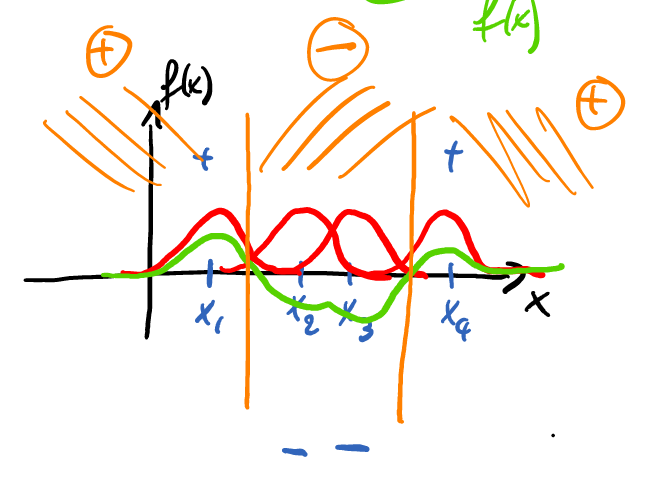
\includegraphics[width=.5\textwidth]{figures/decision_function_kernelized.png}
    \caption{This figure shows that the green line is nothing but a scaled version of the indidiual Gaussian distributions and the associated decision function sign.}
    \label{decision_function_kernelized}
\end{figure}

\subsection{Graphical representations of kernels}

The graphical representation of a sample gaussian and exponential kernel can be found in figures 

\begin{figure}[htbp]
    \centering
    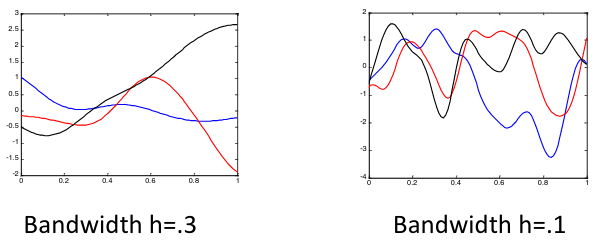
\includegraphics[width=.5\textwidth]{figures/gaussian_kernel.png}
    \caption{Graphical representation of the Gaussian kernel.}
    \label{gaussian_kernel}
\end{figure}

\begin{figure}[htbp]
    \centering
    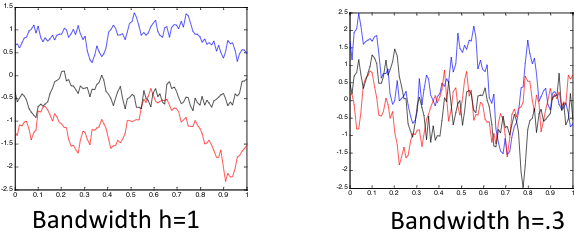
\includegraphics[width=.5\textwidth]{figures/laplacian_kernel.png}
    \caption{Graphical representation of the Laplacian kernel.}
    \label{laplacian_kernel}
\end{figure}

\subsection{Objects where kernels can be used}
The kernels can be defined on a variety of objects:
\begin{itemize}
    \item Sequence kernels
    \item Graph kernels
    \item Diffusion kernels
    \item Kernels on probability distributions
\end{itemize}

Graph kernels can be used for measuring similarity between graphs by comparing random walks on both graphs. They can also be used to measure similarity among nodes in a graph via diffusion kernels not defined here.

\subsection{Kernel engineering}

Suppose we have two kernels:
\begin{equation*}
    k_1:\mathcal{X}\times \mathcal{X}\rightarrow \mathbb{R}\qquad k_2:\mathcal{X}\times \mathcal{X}\rightarrow \mathbb{R}
\end{equation*}
Then the following functions are valid kernels:
\begin{itemize}
    \item $k(\mathbf{x}, \mathbf{x}')=k_1(\mathbf{x}, \mathbf{x}')+k_2(\mathbf{x}, \mathbf{x}')$
    \item $k(\mathbf{x}, \mathbf{x}')=k_1(\mathbf{x}, \mathbf{x}')k_2(\mathbf{x}, \mathbf{x}')$
    \item $k(\mathbf{x}, \mathbf{x}')=ck_1(\mathbf{x}, \mathbf{x}')$ for $c>0$
    \item $k(\mathbf{x}, \mathbf{x}')=f(k_1(\mathbf{x}, \mathbf{x}'))$ where $f$ is a polynomial with positive coefficients or the exponential function.
\end{itemize}

\subsection{The ANOVA kernel}
\begin{equation*}
    k(\mathbf{x}, \mathbf{x}')=\sum_{j=1}^{d}k_j(x_j, x_j')
\end{equation*}
where:
\begin{equation*}
    \mathbf{x}, \mathbf{x}'\in\mathbb{R}^d\qquad k:\mathbb{R}^d\times\mathbb{R}^d\rightarrow \mathbb{R}\qquad  k_j:\mathbb{R}\times\mathbb{R}\rightarrow\mathbb{R}
\end{equation*}
The functions modelled by this kernel can be shown by showing what forms $f(x)$ takes:
\begin{align*}
    f(x) &= \sum_{i=1}^{n}\alpha_i y_i k(x^(i),\mathbf{x})\\
    &= \sum_{i=1}^{n}\alpha_i y_i \sum_{j=1}^{d}k_j(x^(i)_j,\mathbf{x}_j)\\
    &= \sum_{j=1}^{d}\sum_{i=1}^{n}\alpha_i y_i k_j(x^(i)_j,\mathbf{x}_j)\\
    &= \sum_{j=1}^{d}f_j(\mathbf{x}_j)
\end{align*}
which means that the function $f$ decomposes into functions that depend on individual coordinates only, i.e. it is additive decomposition of the function. This property can be useful for high dimensional domains.

\subsection{Modelling pairwise data}

Suppose we have the following two kernels:
\begin{align}
    k((x,z),(x', z')) &= k_x(x,x')\cdot k_z(z,z')\\
    k((x,z),(x', z')) &= k_x(x,x') + k_z(z,z')\\
\end{align}
They can be used to represent the following data:
\begin{figure}[htbp]
    \centering
    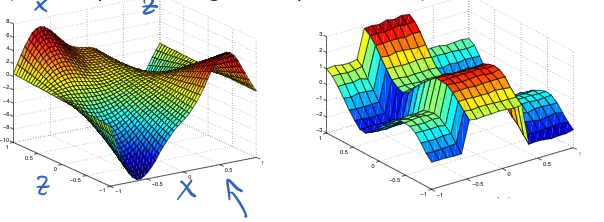
\includegraphics[width=.8\textwidth]{figures/additive_and_multiplicative_effects_of_kernels.png}
    \caption{The left figure can be used to represent a situation where multiplying the kernel could be useful and the right figure can be used to represent a situation where adding the kernel could be useful.}
    \label{additive_and_multiplicative_effects_of_kernels}
\end{figure}

\subsection{Kernels as similarity functions}

Kernels can be used as similarity measures. For instance, consider the Gaussian kernel \\$k(\mathbf{x}, \mathbf{x}')=\exp (-\norm{\mathbf{x}-\mathbf{x}'}^2/h^2)$. If a point $\mathbf{x}$ is close to $\mathbf{x}'$, then the value of $k(\mathbf{x}, \mathbf{x}')\approx 1$, else it is closer to $0$.

\subsection{Comparing k-NN to kernel perceptron}

The prediction for each point in $k$-NN is provided by:
\begin{equation*}
    y=\text{sign}(\sum_{i=1}^{n}y_i\color{blue}[\mathbf{x}\text{ among $k$ nearest neighbors of }\mathbf{x}]\color{black})   
\end{equation*}

As we can see, it compares to the loss of the perceptron:

\begin{equation*}
    y=\text{sign}(\sum_{i=1}^{n}y_i\color{blue}\alpha_ik(\mathbf{x}_i,\mathbf{x})\color{black})   
\end{equation*}
Note: choose $k$ in $k$-NN using cross-validation. 

\begin{table}
    \centering
    \begin{tabular}{lll}
        \toprule
        \textbf{Method} & $k$-NN & Kernelized perceptron\\
        \midrule
        \textbf{Advantages} & No training required & \begin{tabular}{@{}l@{}} Optimized weights can lead to \\ improved performance, can capture \\ global trends with suitable kernels\\ Depends on wrongly classified examples only \end{tabular}\\
        \textbf{Disadvantages} & Depends on all data & Training requires optimisation \\
        \bottomrule
    \end{tabular}
\end{table} 

\subsection{Deriving non-parametric models from parametric ones}

Parametric models have a finite set of paramteters. Examples of such models include linear regression, linear perceptron, etc ...
Nonparametric models grow in complexity with the size of the data. They have the potential to be much more expressive but also more computationally complex. Examples of such models include the kernelized perceptron, $k$-NN, etc... Kernels provide a principled way of deriving non-parametrics models from parametric ones.

\subsection{Kernelized SVM}

The SVM optimization step can be kernelized as follows:
\begin{align*}
    \hat{\mathbf{w}}=\arg\min_{\mathbf{w}}\frac{1}{n}\sum_{i=1}^{n}&\max\left\{0,1-y_i\mathbf{w}^T\mathbf{x}_i\right\}+\lambda\norm{\mathbf{w}}_2^2 \qquad \text{ assuming } \mathbf{w}=\sum_{j=1}^{n}\alpha_jy_jx_j\\
    =&\max\left\{0,1-y_i(\sum_{j=1}^{n}\alpha_jy_jx_j)^Tx_i\right\}\\
    =&\max\left\{0,1-y_i\sum_{j=1}^{n}\alpha_jy_j(x_j^Tx_i)\right\}\\
    =&\max\left\{0,1-y_i\sum_{j=1}^{n}\alpha_jy_jk(x_j, x_i)\right\}\\
    =&\max\left\{0,1-y_i\alpha^Tk_i\right\}\\
\end{align*}
where $k_i=\left[y_1k(\mathbf{x}_i, \mathbf{x}_1), \ldots, y_nk(\mathbf{x}_i, \mathbf{x}_n)\right]^T$ and $\alpha = \left[\alpha_1, \ldots, \alpha_n\right]^T$.

The regularizer can be kernelized as follows:
\begin{align*}
    &\lambda\norm{\mathbf{w}}_2^2\\
    =&\lambda\mathbf{w}\mathbf{w}^T=\lambda(\sum_{i=1}^{n}\alpha_iy_ix_i)^T(\sum_{j=1}^{n}\alpha_jy_jx_j)
    =&\lambda\sum_{i=1}^{n}\sum_{j=1}^{n}\alpha_i\alpha_jy_iy_jx_j^Tx_i\\
    =&\lambda\alpha^T D_y\mathbf{K}D_y\alpha
\end{align*}
where $D_y=\begin{bmatrix}
    y_1 & \ldots & 0\\
    \vdots & \ddots & \vdots\\
    0 & \ldots & y_n\\
\end{bmatrix}$ and $\mathbf{K} = \begin{bmatrix}
    k(x_1,x_1) & \ldots & k(x_1,x_n)\\
    \vdots & \ddots & \vdots\\
    k(x_n,x_1) & \ldots & k(x_n,x_n)\\
\end{bmatrix}$

\subsection{Kernelizing linear regression}

Original parametric linear regresion optimization problem is stated as follows:
\begin{equation*}
    \hat{\mathbf{w}}=\arg\min_{\mathbf{w}}\frac{1}{n}\sum_{i=1}^{n}(\mathbf{w}^T\mathbf{x}_i-y_i)^2+\lambda\norm{\mathbf{w}}_2^2
\end{equation*}

We kernelize linear regression in two parts:

\begin{align*}
    =& \sum_{i=1}^{n}(\mathbf{w}^T\mathbf{x}_i-y_i)^2\\
    =& \sum_{i=1}^{n}((\sum_{j=1}^{n}\alpha_jx_jx_i)^T\mathbf{x}_i-y_i)^2\\
    =& \sum_{i=1}^{n}(\sum_{j=1}^{n}\alpha_j(x_j^Tx_i)\mathbf{x}_i-y_i)^2\\
    =& \sum_{i=1}^{n}(\sum_{j=1}^{n}\alpha_j(x_j^Tx_i)\mathbf{x}_i-y_i)^2\\
    =& (\alpha^2k_i-y_i)^2
\end{align*}
and 

\begin{align*}
    =& \sum_{i=1}^{n}\sum_{j=1}^{n}\alpha_i\alpha_jx_i^Tx_j\\
    =& \alpha^T\mathbf{K}\alpha
\end{align*}
hence we have:
\begin{align*}
    \hat{\alpha}&=\arg\min_{\alpha\in\mathbb{R^n}}\frac{1}{n}\sum_{i=1}^{n}(\alpha^Tk_i-y_i)^2+\lambda\alpha^T\mathbf{K}\alpha\\
    \hat{\alpha}&=\arg\min_{\alpha\in\mathbb{R^n}}\frac{1}{n}\norm{\alpha^T\mathbf{K}-\mathbf{y}}_2^2+\lambda\alpha^T\mathbf{K}\alpha
\end{align*}
which has a closed-form solution:
\begin{equation*}
    \hat{\alpha}=(\mathbf{K}+n\lambda \mathbf{I})^{-1}\mathbf{y}
\end{equation*} 
For prediction, given a data point $\mathbf{x}$, we predict the response $y$ as:
\begin{equation*}
    \hat{y}=\sum_{i=1}^{n}\hat{\alpha_i}k(\mathbf{x_i},\mathbf{x})
\end{equation*}

\subsubsection{Application: semi-parametric regression}

Often, parametric models are too rigid and non-parametric models fail to extrapolate. The solution to this problem is to use additive combination of linear and non-linear kernel function as shown below:

\begin{equation*}
    k(\mathbf{x}, \mathbf{x}') = c_1\exp\left(\norm[]{\mathbf{x} - \mathbf{x}'}_2^2/h^2\right) + c_2\mathbf{x}^T\mathbf{x}'
\end{equation*}

The decision function is then defined as follows:

\begin{align*}
    f(\mathbf{x}) &= \sum_{i=1}^{n}\alpha_i k(\mathbf{x}_i, \mathbf{x})=\sum_{i=1}^{n}\left(\alpha_i(c_i \exp(-\norm[]{\mathbf{x}_i-\mathbf{x}}_2^2/h^2))+c_2\mathbf{x}_i\mathbf{x}'\right)\\
    &= c_1 \sum_{i=1}^{n}\alpha_i k(\mathbf{x}_i,\mathbf{x}) = \sum_{i=1}^{n}\left(\alpha_i(c_1\exp\left(\norm[]{\mathbf{x_i-\mathbf{x}}_2^2/h^2}\right))+c_2\mathbf{x}_i^T\mathbf{x}'\right)\\
    &= c_1\sum_{i=1}^{n}\alpha_i\exp\left(-\norm{\mathbf{x}_i-\mathbf{x}}_2^2/h^2\right) + \left(c_2\sum_{i=1}^{n}\alpha_ix_i\right)^T\mathbf{x}
    &= f_1(\mathbf{x})+\mathbf{w}^T\mathbf{x}
\end{align*}

The efficiency of this methodology can be seen in the figure \ref{semiparametricregression}.

\begin{figure}[htbp]
    \centering
    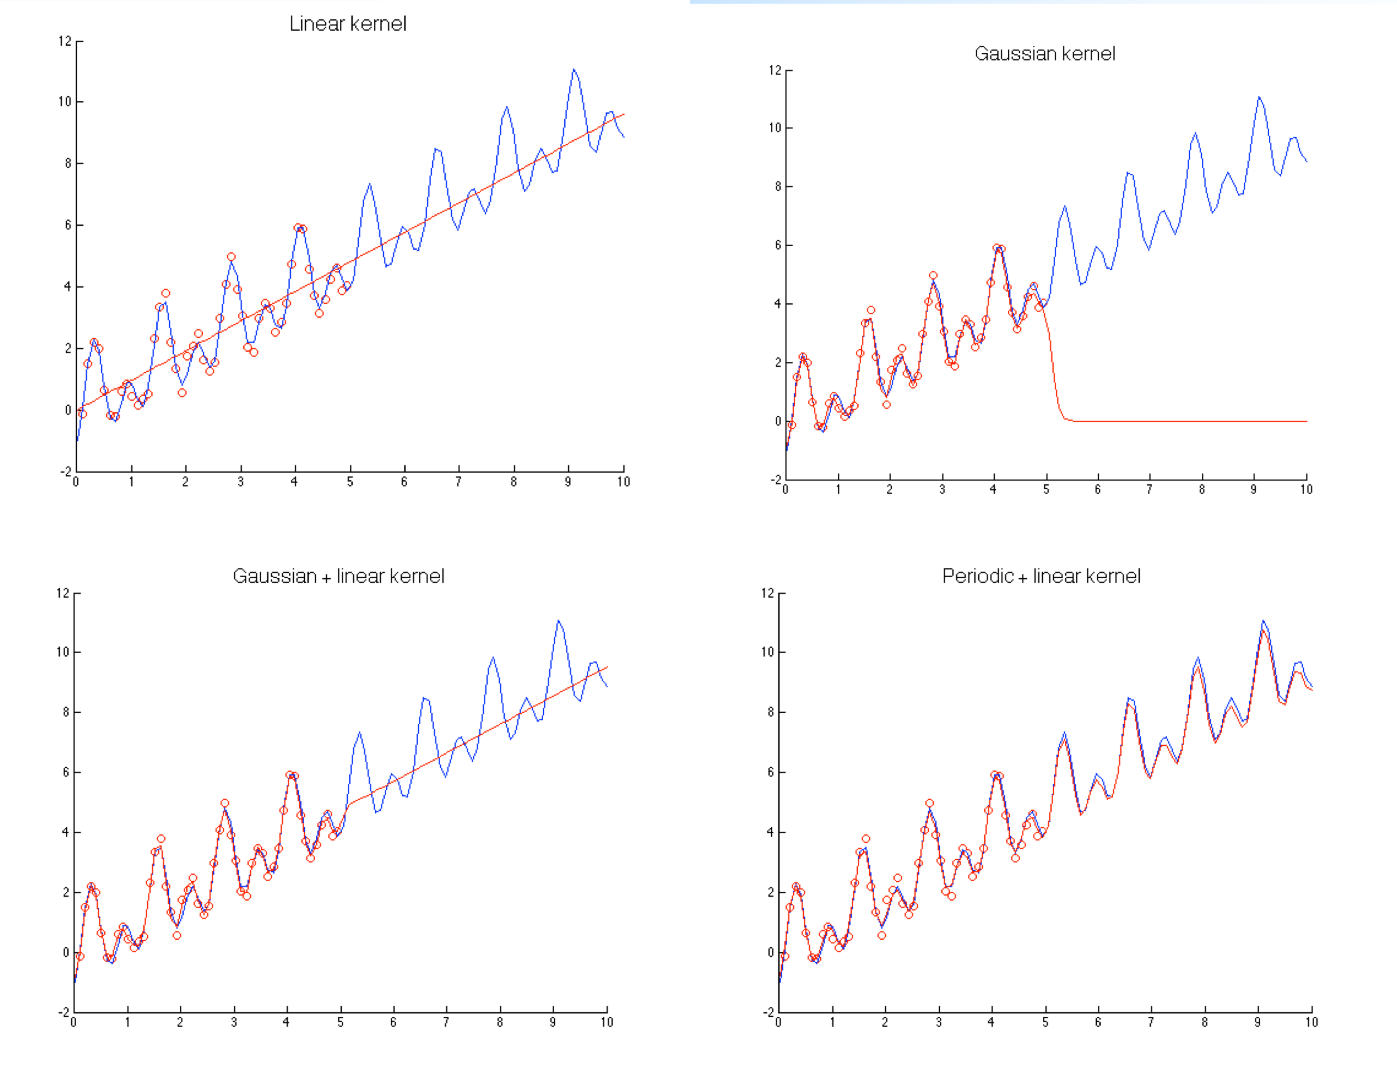
\includegraphics[width=.5\textwidth]{figures/semi-parametric-regression.png}
    \caption{Various learned models overlayed with the function that we wish to learn based on the available data. Clearly, a linear kernel and a periodic parametric model seem to fit best the pattern observed.}
    \label{semiparametricregression}
\end{figure}

This approach can be used to design P450 chimeras, predict protein fitness landscapes, and various other protein engineering applications.

\subsection{Choosing kernels \& risk of overfitting}

Choosing correct kernels is a combination of domain knowledge, brute force or heuristic search using cross-validation. Since kernels map to very high dimensional spaces, it is difficult to see what we hope to be able to learn. Typically the number of parameters is drastically smaller than the number of dimensions. One way of tackling this problem is to set the number of parameters equal to that of the number of datapoints, which in this case would be called non-parametric learning. Another way of tackling this problem is to use regularization, which is built into kernelized linear regression and SVMs but not into the kernelized Perceptron. Recall the formulations of KLR and SVM:
\begin{align*}
    \hat{\alpha} &= \arg\min_{\alpha}\frac{1}{n}\norm[]{\alpha^T\mathbf{K}=\mathbf{y}}_2^2+\lambda\alpha^T\mathbf{K}\alpha\\
    \hat{\alpha} &= \arg\min_{\alpha}\frac{1}{n}\sum_{i=1}^{n}\max\left\{0,1-y_i\alpha^T\mathbf{k}_i\right\} + \lambda\alpha^T\mathbf{D}_{\mathbf{y}}\mathbf{K}\mathbf{D}_\mathbf{y}\alpha
\end{align*}

\section{Class imbalance}

Often data looks very imbalanced, e.g. there are more false negatives than false positives, see figure \ref{imbalanced_data}. Sources of imbalanced data include fraud detection datasets, spam filtering, process monitoring, medical diagnosis, feedback in recommender systems. The main issues related with imbalanced data include \textit{performance metrics}, where the performance assessment of the model is not a good metric. It may be good to prefer certain mistakes over others, i.e. we trade false positives for false negatives. The minority class instance contribute little to the empirical risk. It therefore may be ignored during optimization. There are two solutions to the problem of imbalanced datasets:
\begin{itemize}
    \item \textbf{Subsampling}: this entails removing examples from the majority class (e.g. uniformly at random) such that the resulting dataset is balanced. 
    \item \textbf{Upsampling}: this entails repeating data points from the minority class, possibly with small random perturbation to obtain a balanced data set.
    \item It's also a possibility to use cost-sensitive classification methods to deal with these issues.
\end{itemize}

Illustrations of these two approaches are shown in figure \ref{up_and_downsampling}.

\begin{figure}
    \centering
    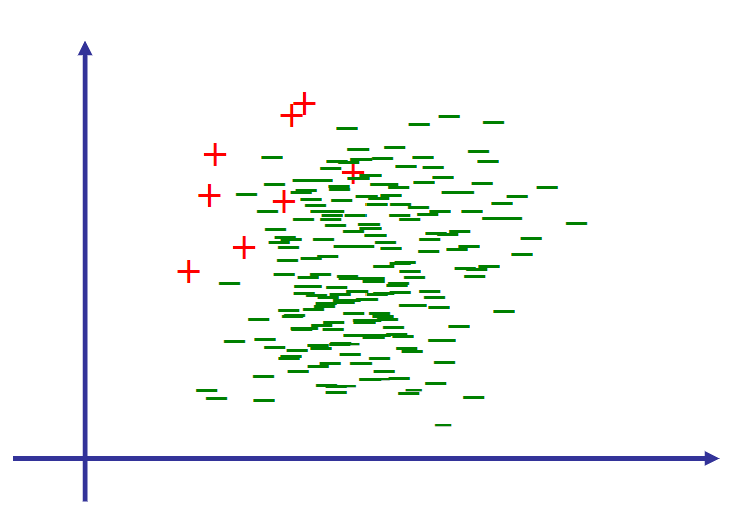
\includegraphics[width=.5\textwidth]{figures/imbalanced_data.png}
    \caption{Example of a dataset with imbalanced data.}
    \label{imbalanced_data}
\end{figure}

\begin{figure}
    \centering
    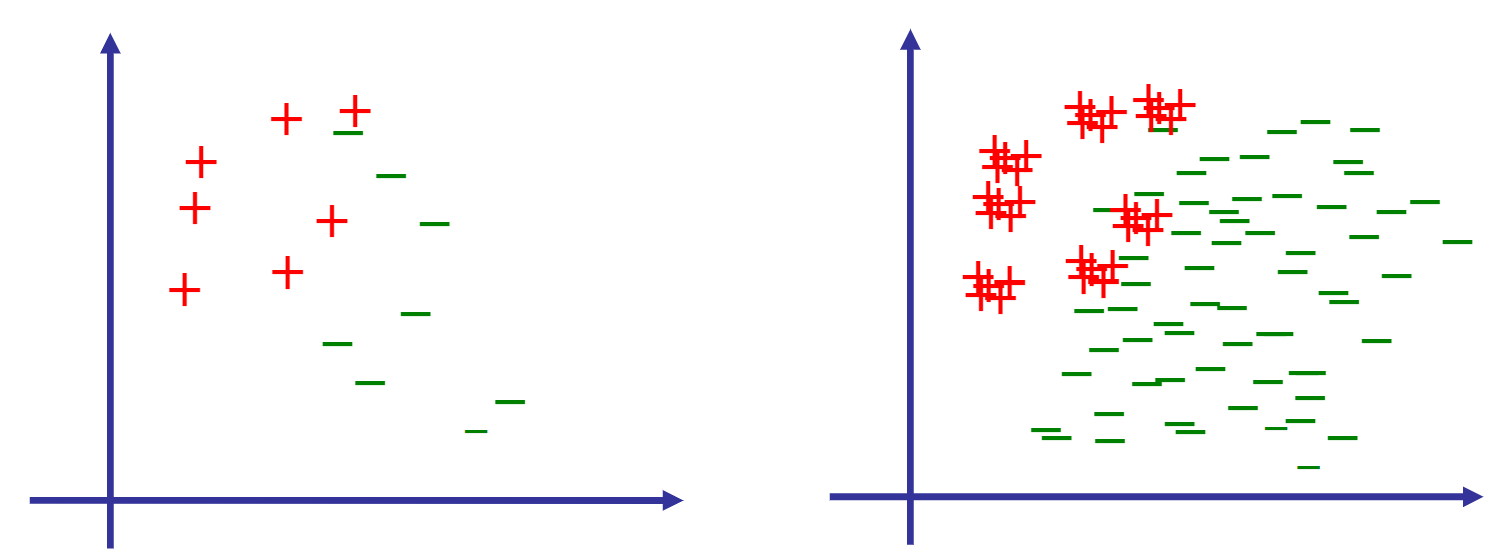
\includegraphics[width=.5\textwidth]{figures/up_and_down_sampling.png}
    \caption{Illustration of subsampling (left) and upsampling (right).}
    \label{up_and_downsampling}
\end{figure}

\subsection{Cost-sensitive classification}

This entails modifying the perceptron/SVM to take class balance into account. The only different is in the cost function, where we add a class coefficient in front of the loss function:
\begin{equation*}
    \ell_{CS}(\mathbf{w};\mathbf{x},y)=\color{blue}c_y\color{black}\ell(\mathbf{w};\mathbf{x},y)
\end{equation*}
For the perceptron, this becomes
\begin{equation*}
    \ell_{CS}(\mathbf{w};\mathbf{x},y)=\color{blue}c_y\color{black}\max(0,-y\mathbf{w}^T\mathbf{x})
\end{equation*}
For the SVM, this becomes
\begin{equation*}
    \ell_{CS}(\mathbf{w};\mathbf{x},y)=\color{blue}c_y\color{black}\max(0,1-y\mathbf{w}^T\mathbf{x})
\end{equation*}
where, in all cases, $c_+, c_->0$ control the tradeoff to be made.

An illustration of the adapted cost function can be seen in figure \ref{perceptron-class-sensitive-loss}.

\begin{figure}
    \centering
    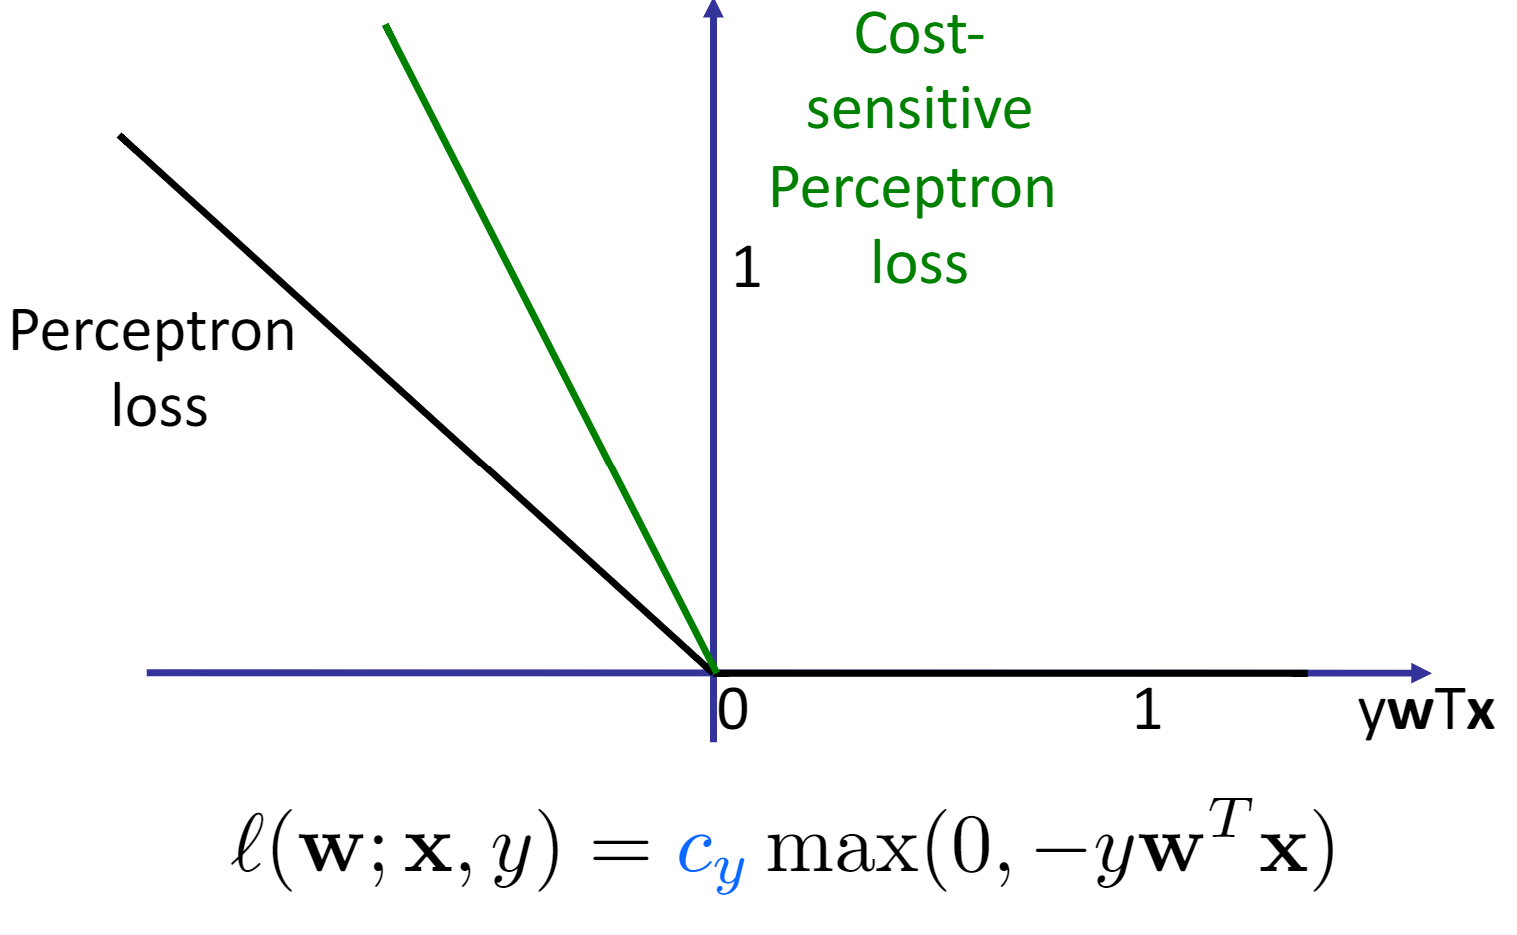
\includegraphics[width=.5\textwidth]{figures/perceptron-class-sensitive-loss.png}
    \caption{Perceptron loss}
    \label{perceptron-class-sensitive-loss}
\end{figure}

\subsection{Avoiding redundancy}

Given that the empirical loss, given by:
\begin{align*}
    \hat{R}(\mathbf{w};c_+,c_-) &= \frac{1}{n}\sum_{i_{y_i=1}}c_+\ell(\mathbf{w};x_i,y_i)+\frac{1}{n}\sum_{i_{y_i=1}}c_-\ell(\mathbf{w};x_i,y_i)\\
    \forall\alpha>0:\hat{R}(\mathbf{w};\alpha c_+, \alpha c_-) &=\alpha\hat{R}(\mathbf{w};c_+,c_-)\\
    \Rightarrow \arg\min_{\mathbf{w}}\hat{R}(\mathbf{w};\alpha c_+, \alpha c_-)&=\arg\min_{\mathbf{w}}\alpha \hat{R}(\mathbf{w}; c_+, c_-)=\arg\min_{\mathbf{w}}\alpha \hat{R}(\mathbf{w}; \frac{c_+}{c_-}, 1)\\
    \Rightarrow \text{w.l.o.g.: } \alpha&=\frac{1}{c_{-}}.
\end{align*}

Which basically means that the tradeoff to make for imbalanced datasets can be determined by one parameter.

\subsection{Metrics for imbalanced datasets}

A generally inappropriate metric for imbalanced datasets is accuracy, defined as 
\begin{equation*}
    \text{Accuracy} = \frac{TP+TN}{TP+TN+FP+FN}=\frac{TP+TN}{N}
\end{equation*}
Other, more suitable metrics include:
\begin{equation*}
    \text{Precision}=\frac{TP}{TP+FP}=\frac{TP}{P+}
\end{equation*}
\begin{equation*}
    \text{Recall}=\text{True positive rate (TPR)}=\frac{TP}{TP+FN}=\frac{TP}{N+}
\end{equation*}
\begin{equation*}
    \text{F1 score}=\frac{2TP}{2TP+FN+FP}=\frac{2}{\frac{1}{\text{Prec}}+\frac{1}{\text{Rec}}}
\end{equation*}
\begin{equation*}
    \text{False positive rate (FPR)} = \frac{FP}{TN+FP}
\end{equation*}
An interesting observation to make is that given the probability $p$ of observing a positive sample, we have:
\begin{align*}
    \mathbb{E}[\text{TPR}]&=\frac{\mathbb{E}[\text{TP}]}{n_+}=\frac{p\cdot n_+}{n_+}=p\\
    \mathbb{E}[\text{TPR}]&=\frac{\mathbb{E}[\text{TP}]}{n_-}=\frac{p\cdot n_-}{n_-}=p
\end{align*}

The receiver operator characteristic (ROC) curve (see figure \ref{roc-curve}) can also be used to make an assessment of a classifier.

\begin{figure}
    \centering
    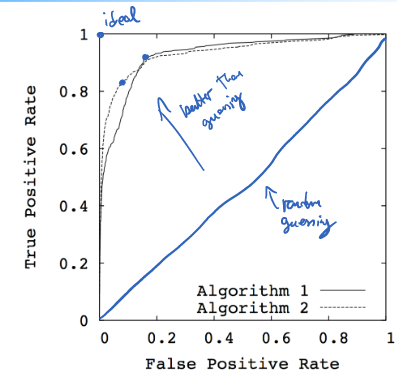
\includegraphics[width=.5\textwidth]{figures/roc_curve.png}
    \caption{}
    \label{roc-curve}
\end{figure}

Note that a performance measure associated to the precision recall curve is the area under the curve. A random classifier has an AUC of 0.5 and an ideal classifier has an AUC of 1.s

It is also important that the confusion matrix itself is also often used to evaluate the performance of a binary or even multi-class classifier.

\begin{table}
    \centering
    \renewcommand\arraystretch{1.5}
    \setlength\tabcolsep{0pt}
    \begin{tabular}{c >{\bfseries}r @{\hspace{0.7em}}c @{\hspace{0.4em}}c @{\hspace{0.7em}}l}
      \multirow{10}{*}{\parbox{1.1cm}{\bfseries\raggedleft actual\\ value}} & 
        & \multicolumn{2}{c}{\bfseries Prediction outcome} & \\
      & & \bfseries p & \bfseries n & \bfseries total \\
      & p$'$ & \MyBox{True}{Positive} & \MyBox{False}{Negative} & P$'$ \\[2.4em]
      & n$'$ & \MyBox{False}{Positive} & \MyBox{True}{Negative} & N$'$ \\
      & total & P & N &
    \end{tabular}        
\end{table}

\subsection{Obtaining the optimal tradeoff}

Two ways of obtaining a good tradeoff is to either use a cost sensitive classifier and vary the tradeoff parameter. The second option is to find a single classifier and vary the classification threshold $\tau$ in the following formula:
\begin{equation*}
    y=\text{sign}(\mathbf{w}^T\mathbf{x}-\tau)
\end{equation*}

The optimal value for the threshold can be determined using the precision-recall curve \ref{precision-recall-curve}. 

\begin{figure}
    \centering
    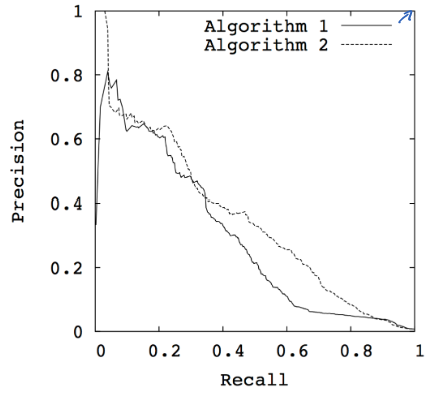
\includegraphics[width=.5\textwidth]{figures/precision_recall_curve.png}
    \caption{An example of a precision-recall curve.}
    \label{precision-recall-curve}
\end{figure}

An interesting note to make in terms of the relationship between the ROC curve and the precision recall curve is captured in the following theorem:

\begin{theorem}
    Algorithm 1 dominates Algorithm 2 in terms of ROC curve $\Leftrightarrow$ Algorithm 1 dominates Algorithm 2 in terms of precision recall curve.
\end{theorem}

\section{Multiclass problems}

A multiclass problem is defined as follows. Given a dataset $\mathcal{D}={(\mathbf{x}_1, y_1),\ldots, (\mathbf{x}_n, y_n)}$ for $y_i\in{1,\ldots, c}$, we want a function $f:\mathcal{X}\rightarrow \mathcal{Y}$ where $y_i\in\mathcal{Y}={1,\ldots,c}$ and $\mathbf{x}_i\in\mathcal{X}\subseteq\mathbb{R}^d$, as illustrated in figure \ref{multiclass-problem}.

\begin{figure}
    \centering
    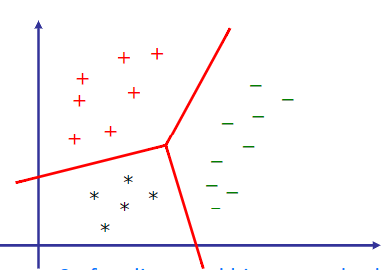
\includegraphics[width=.5\textwidth]{figures/multiclass-problem.png}
    \caption{Illustration of a multiclass problem.}
    \label{multiclass-problem}
\end{figure}

\subsection{One-vs-all}

One approach to solve the problem is to solve $c$ binary classifiers, i.e. one for each class, where all positive samples are from class i and all negative samples represent all other points. We then classify using the classifier with the largest confidence. In other words, we fit $f^{(i)}:\mathcal{X}\rightarrow\mathbb{R}$ and $f^{(i)}(x)=\mathbf{w}^{(i)T}\mathbf{x}$ and we predict $\hat{y}=\arg\max_{i}f^{(i)}(\mathbf{x})=\arg\max_{i}\mathbf{w}^{(i)T}\mathbf{x}$. 

\subsubsection{Confidence in a classification}

The confidence in a classification decision can be visualized as in figure \ref{confidence-in-classification}. For $\alpha>0$, we have 
\begin{equation*}
    \text{sign}((\alpha\mathbf{w})^T\mathbf{x})=\text{sign}(\mathbf{w}^T\mathbf{x})
\end{equation*}

Thus although $\alpha\mathbf{w}$ and $\mathbf{w}$ implement the same decision boundary, they have a different confidence level. There are two solutions to this problem: 
\begin{enumerate}
    \item $\mathbf{w}\leftarrow \frac{\mathbf{w}}{\norm{\mathbf{w}}_2}$, i.e. this is normalized to unit length.
    \item In practice, when using regularization, the magnitude of $\norm[]{\mathbf{w}}_2$ is kept under control. 
\end{enumerate} 

\begin{figure}
    \centering
    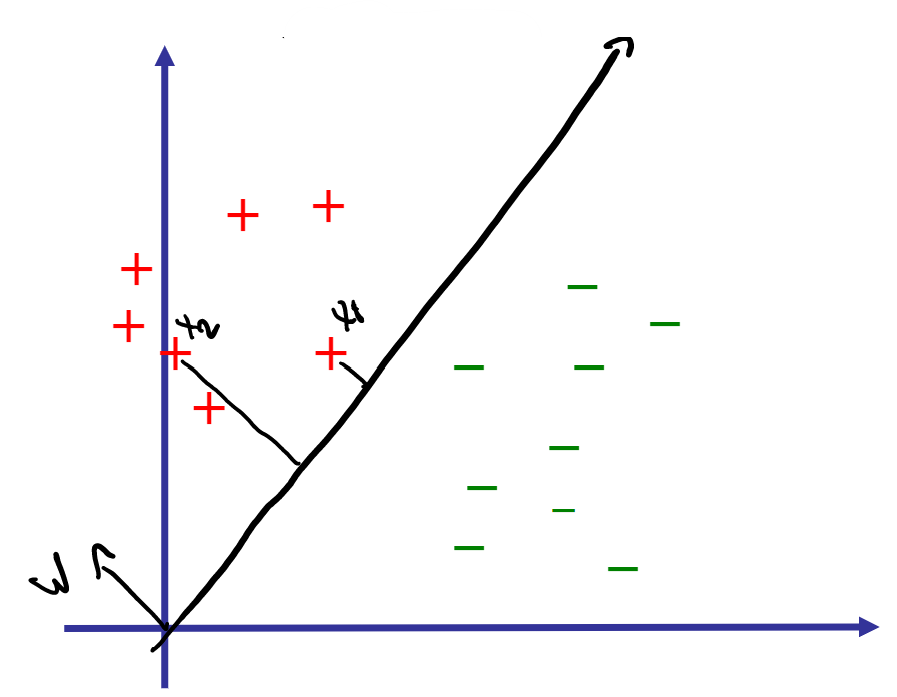
\includegraphics[width=.5\textwidth]{figures/confidence-in-classification.png}
    \caption{Illustration of the confidence in classification. We see that $\mathbf{w}^T\mathbf{x}_2>\mathbf{w}^T\mathbf{x}_1$ so that means that the label + is given with more confidence to $\mathbf{x}_2$ than for $\mathbf{x}_1$}
    \label{confidence-in-classification}
\end{figure}

The decision boundary of the one-vs-all decision can be represented as in figure \ref{ova-decision-boundary}. 

\begin{figure}
    \centering
    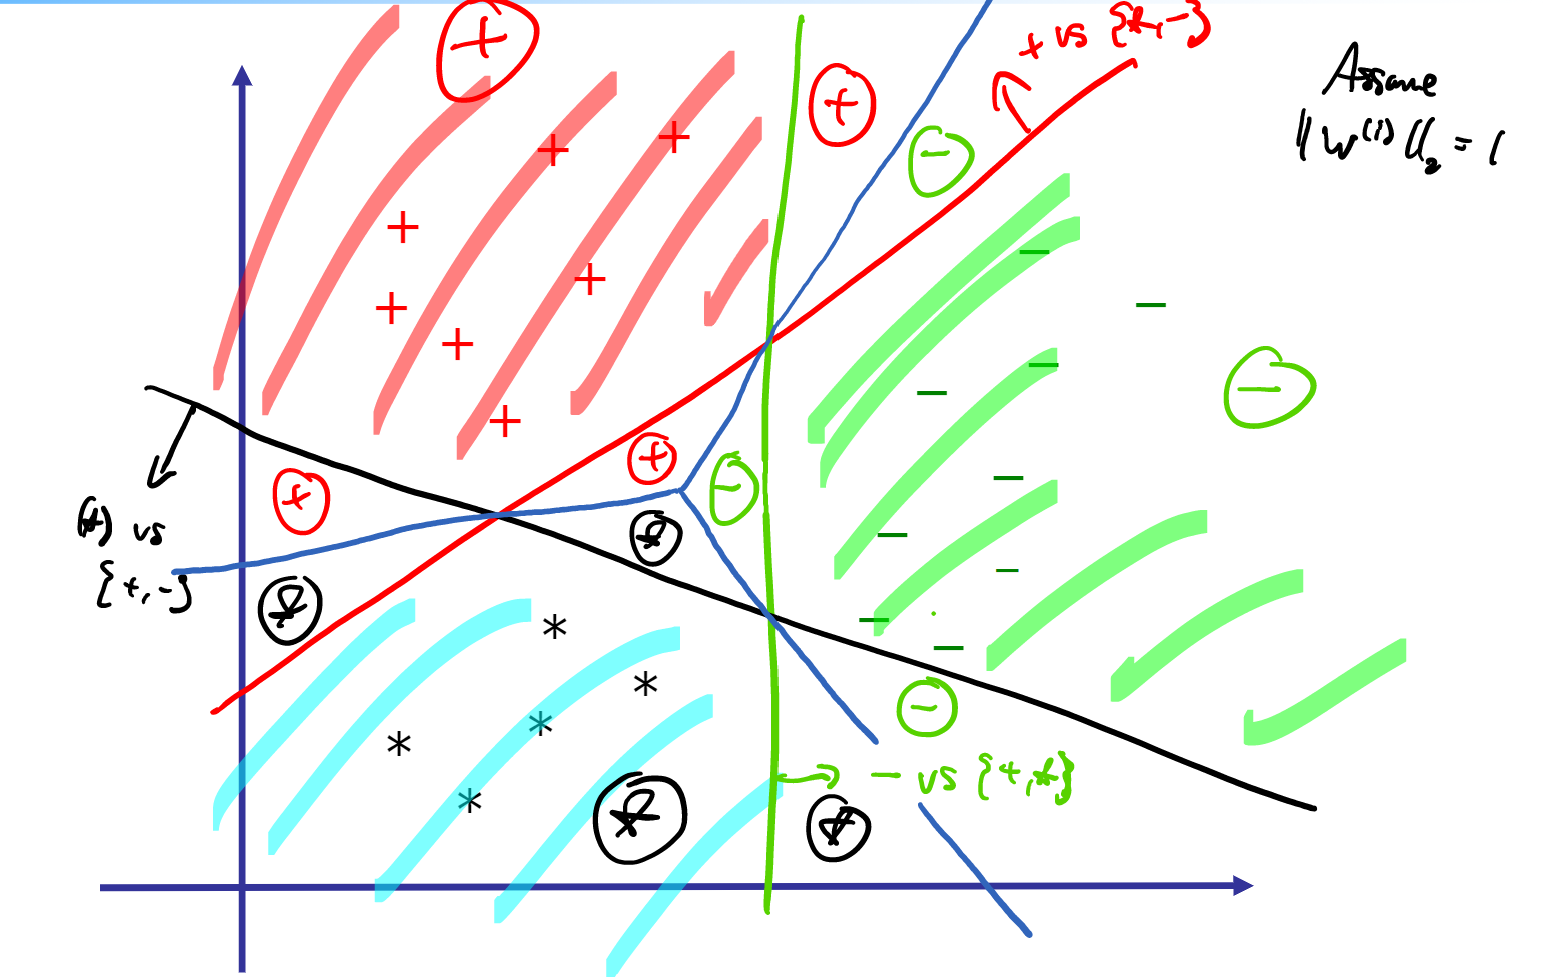
\includegraphics[width=.5\textwidth]{figures/ova-decision-boundary.png}
    \caption{One-vs-all decision boundary.}
    \label{ova-decision-boundary}
\end{figure}

\subsubsection{Challenges}
There are several challenges associated with the one-vs-all technique:
\begin{itemize}
    \item It only works if classifiers produce confidence scores on the same scale.
    \item Individual binary classifier see imbalanced data, even if the whole data set is balanced.
    \item One class might not be linearly separable from all other classes.
\end{itemize}

\subsection{One-vs-one}

The idea is to train $c(c-1)/2$ binary classifiers, one for each pair of classes $(i,j)$. Positive examples contain all points from class $i$ and negative examples contain all points from class $j$. Then, we apply a voting scheme, i.e. the class with the highest number of positive prediction wins. A graphical representation of the one-vs-one classification is shown in figure \ref{one-vs-one}.

\begin{figure}
    \centering
    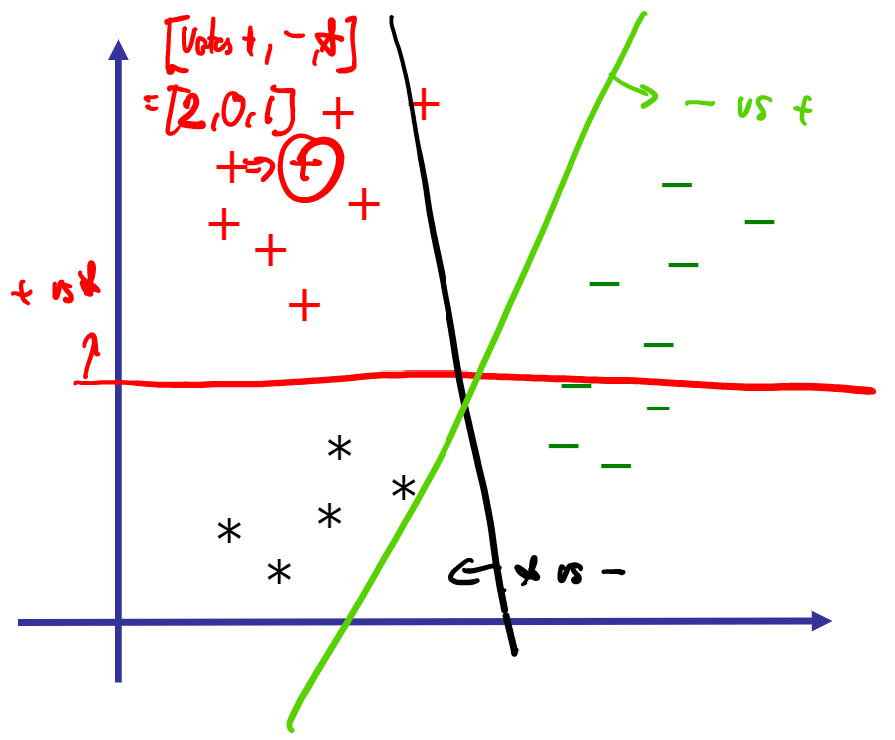
\includegraphics[width=.5\textwidth]{figures/one-vs-one.png}
    \caption{Illustration of the one-vs-one classification technique. Here, we see that each decision boundary is fit for each pair of classes ($i,j$).}
    \label{one-vs-one}
\end{figure}

\begin{table}
    \centering
    \begin{tabular}{lll}
        \toprule
        \textbf{Method} & \textit{One-vs-all} & \textit{One-vs-one} \\ 
        \midrule
        \textbf{Advantages} & Only $c$ classifiers needed (faster!) & No confidence needed\\
        \textbf{Disadvantages} & Requires confidence + leads to class imbalance & Need to train $c(c-1)/2$)\\
        \bottomrule
    \end{tabular}
\end{table}

\subsection{Encodings}

There are other methods to tackle multiclass problems, e.g. using other encodings (error correcting output codes). There are also other explicit multiclass models, such as the multi-class perceptron/svm etc. Some models are naturally multi-class, such as nearest neighbors, generative probabilistic models, etc. However, one should keep in mind that one-vs-all/one-vs-one usually works very well. 

A way to reduce the number of classes we need to work with can be reduce by using an encoding. The length of the encoding will then scale with the $log_{2}c$, see table \ref{binary-label-encoding}. Then in principle the multiclassfication problem is phrased as a decoding task of the class label, where each classifier predicts one bit, which in this case we would get away with $\mathcal{O}(\log c)$ classifiers. In this case, ideas from coding theory to do multi-class classification can be used to do multi-class classification.

\begin{table}
    \centering
    \begin{tabular}{cc}
        \toprule
        \textit{Class} & \textit{Encoding} \\
        \midrule
        0 & [0,0,0,0]\\
        1 & [0,0,0,1]\\
        2 & [0,0,1,0]\\
        \vdots & \vdots\\
        $c-1$ & [1,1,1,1]\\
        \bottomrule
    \end{tabular}
    \caption{Table containing the class name and corresponding encoding}
    \label{binary-label-encoding}
\end{table}

\subsection{Multi-class SVMs}

The key idea of multi-class SVMs is to maintain $c$ weight vectors $\mathbf{w}^{1},\ldots,\mathbf{w}^{c}$, one for each class. Then we predict using:
\begin{equation*}
    \hat{y} \leftarrow \arg\max_{i\in{1,\ldots,c}}\mathbf{w}^{(i)T}\mathbf{x}
\end{equation*}
Given each data point $(\mathbf{x},y)$, we want to achieve that:
\begin{align}\label{multiclasssvm}
    \mathbf{w}^{(y)}\mathbf{x}&\geq\mathbf{w}^{(i)}\mathbf{x}+1 \forall i\in\left\{1,\ldots, c\right\}\setminus{y}\\
    \equiv \mathbf{w}^{(y)}\mathbf{x}&\geq\max_{i\in\left\{1,\ldots,c\right\}\setminus\left\{y\right\}}\mathbf{w}^{(i)}\mathbf{x}+1
\end{align}

\subsection{Multi-class Hinge loss}

\begin{equation*}
    \ell_{MC-H}(\mathbf{w}^{1},\ldots, \mathbf{w}^{c};\mathbf{x}, y)=\max(0,1+\max_{j\in\left\{1,\ldots, y-1,y+1, \ldots,c\right\}} \mathbf{w}^{(j)T}\mathbf{x}-\mathbf{w}^{(y)T}\mathbf{x})
\end{equation*}
which is equal to 0 when equation \ref{multiclasssvm} is satisfied. 

The gradient of the Hinge loss is then defined as:
\begin{equation*}
    \nabla_{w^{(i)}}\ell_{MC-H}(\mathbf{w}^{(1:c)};\mathbf{x},y) = \begin{cases}
        0 \text{ if equation \ref{multiclasssvm} is satisfied or } i\neq y\land i\neq \arg\max_{j}\mathbf{w}^{(j)T}\mathbf{x}\\
        -\mathbf{x} \text{ if \ref{multiclasssvm} is not satisfied and } i=y\\
        +\mathbf{x} \text{ otherwise.}
    \end{cases}
\end{equation*}

\section{Neural networks}

\subsection{Importance and characteristics of features}

Succes in learning crucially depends on the quality of features. Hand-designing features however requires domain knowledge. However, kernels could be used to engineer features as they provide a rich set of feature maps, they can fit almost any function with infinite data. However, choosing the right kernel can be challenging and the computational complexity grows exponentially with the size of the data. The question then becomes whether or not we can learn good features from the data directly. The overall objective function for neural networks to optimize is the following:
\begin{equation*}
    \mathbf{w}* =\arg\min_{\mathbf{w}}\sum_{i=1}^{n}\ell(y_i;\sum_{j=1}^{m}w_j\phi_j(\mathbf{x}_j))=\arg\min_{\mathbf{w}}\sum_{i=1}^{n}\ell(y_i;f_i)
\end{equation*}
where $\ell(y_i,f_i)$ is usually defined as $\ell(y_i,f_i)=(y_i-f_i)^2$ (squared loss). A key idea then is to parametrize the feature maps, and optimize over the parameters, i.e. our optimization objective is to tune both the parameters and the weights to minimize the loss:
\begin{equation*}
    \mathbf{w}*=\arg\min_{\mathbf{w},\mathbf{\theta}}\sum_{i=1}^{n}\ell(y_i;\sum_{j=1}^{m}w_j\phi(\mathbf{x}_i,\mathbf{\theta}))
\end{equation*}
One possibility of achieving this optimization is to define the following feature map:
\begin{equation*}
    \phi(\mathbf{x},\mathbf{\theta})=\varphi(\mathbf{\theta}^T\mathbf{x})
\end{equation*}
where $\mathbf{\theta}\in\mathbb{R}^d$ and $\phi:\mathbb{R}\rightarrow\mathbb{R}$ is a nonlinear function, called an \textit{activation function}.
An example of such an activation function is the sigmoid and tanh activation functions. The signmoid function is given by:
\begin{equation*}
    \varphi(z)=\frac{1}{1+\exp(-z)}
\end{equation*}
The tanh function is given by:
\begin{equation*}
    \varphi(z)=\tanh(z)=\frac{exp(z)-\exp(-z)}{exp(z)+\exp(-z)}
\end{equation*}
The rectified linear unit is also often used, which is defined as:
\begin{equation*}
    \phi(z)=\max(z,0)
\end{equation*}
The decision function of an artificial neural network is of the form:
\begin{equation*}
    f(\mathbf{x}_i; \mathbf{w}, \mathbf{\theta})=\sum_{j=1}^{m}w_j\varphi(\theta^T_j\mathbf{x})=\sum_{j=1}^{m}w_jv_j
\end{equation*}
More generally, the term artificial neural network refers to nonlinear functions which are nested compositions of variable linear functions composed with fixed nonlinearities.
\subsection{Graphical representation}
A neural network can be represented as shown in figure \ref{graphical-representation-ann}
\begin{figure}
    \centering
        \begin{tikzpicture}[
            init/.style={
            draw,
            circle,
            inner sep=2pt,
            font=\Huge,
            join = by -latex
            },
            squa/.style={
            draw,
            inner sep=2pt,
            font=\Large,
            join = by -latex
            },
            start chain=2,node distance=13mm
            ]
            \node[on chain=2] 
            (x2) {$x_2$};
            \node[on chain=2,join=by o-latex] 
            {$w_2$};
            \node[on chain=2,init] (sigma) 
            {$\displaystyle\Sigma$};
            \node[on chain=2,squa,label=above:{\parbox{2cm}{\centering Activate \\ function}}]   
            {$f$};
            \node[on chain=2,label=above:Output,join=by -latex] 
            {$y$};
            \begin{scope}[start chain=1]
            \node[on chain=1] at (0,1.5cm) 
            (x1) {$x_1$};
            \node[on chain=1,join=by o-latex] 
            (w1) {$w_1$};
            \end{scope}
            \begin{scope}[start chain=3]
            \node[on chain=3] at (0,-1.5cm) 
            (x3) {$x_3$};
            \node[on chain=3,label=below:Weights,join=by o-latex] 
            (w3) {$w_3$};
            \end{scope}
            \node[label=above:\parbox{2cm}{\centering Bias \\ $b$}] at (sigma|-w1) (b) {};
            
            \draw[-latex] (w1) -- (sigma);
            \draw[-latex] (w3) -- (sigma);
            \draw[o-latex] (b) -- (sigma);
            
            \draw[decorate,decoration={brace,mirror}] (x1.north west) -- node[left=10pt] {Inputs} (x3.south west);
        \end{tikzpicture}
    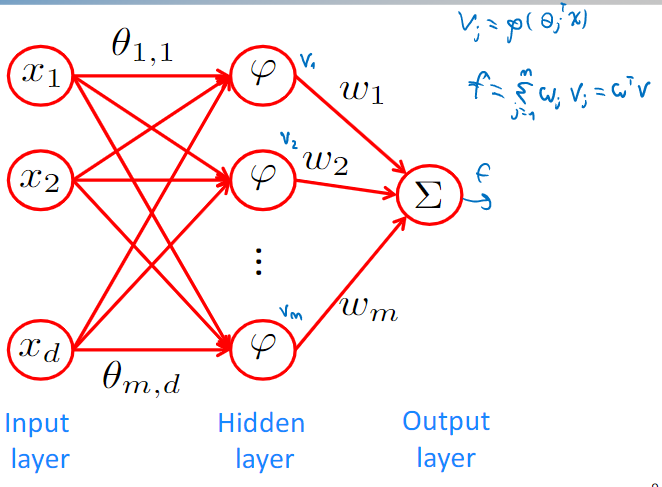
\includegraphics[width=.5\textwidth]{figures/ann-graph-representation.png}
    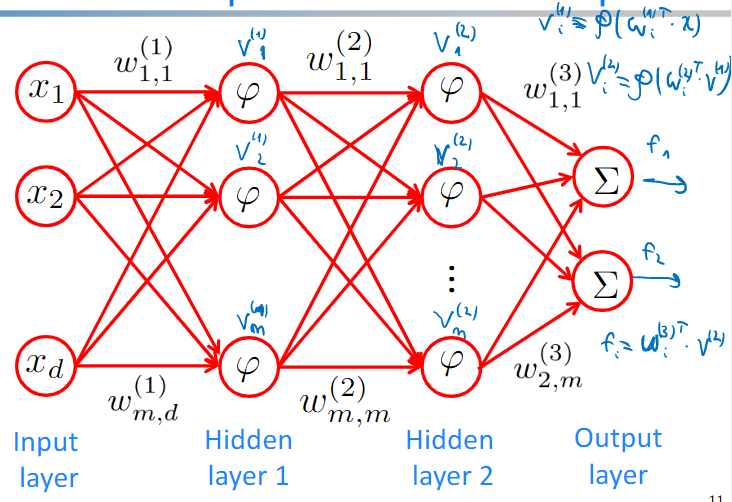
\includegraphics[width=.5\textwidth]{figures/two-layer-ann-representation.png}
    \caption{Graphical representations of an artificial neural network.}
    \label{graphical-representation-ann}
\end{figure}
Note that neural networks can have multiple outputs for multi-class prediction (one output per class or multi-output regression). They can also have more than one hidden layer -- networks with large amounts of neural networks with several hidden layers are called deep neural networks. Indexing in neural networks is done as shown in figure \ref{indexing-ann}.

\begin{figure}
    \centering
    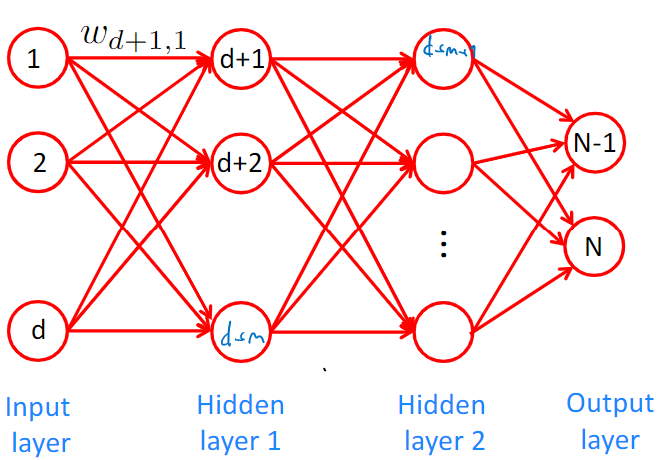
\includegraphics[width=.5\textwidth]{figures/indexing-ann.png}
    \caption{Indexing convention of ANNs}
    \label{indexing-ann}
\end{figure}

\subsection{Making predictions using ANNs}
Suppose we have learned all paramters $w_{i,j}$. Given an input, we now make predictions using forward propagation. The forward propagation procedure is described as follows:
\begin{enumerate}
    \item For each unit $j$ on the input layer, we set its value to $v_j=x_j$.
    \item For each layer $\ell=1:L-1$
    \begin{enumerate}
        \item For each unit $j$ on layer $\ell$ we set its value:
        \begin{equation*}
            v_j=\varphi\left(\sum_{i\in\text{Layer}_{\ell-1}}w_{j,i}v_i\right)
        \end{equation*}
    \end{enumerate}
    \item For each unit $j$ on output layer, set its value:
    \begin{equation*}
        f_j=\sum_{i\in\text{Layer}_{L-1}}^{w_{j,i}v_i}
    \end{equation*}
    \item Predict $y_j=f_j$ for regression, and $y_j=\text{sign}(f_j)$ for regression. For multiclass problems, the prediction is made as $\hat{y}=\arg\max_{j}f_j$.
\end{enumerate}

Another way of writing the forward propagation algorithm is as follows:
\begin{enumerate}
    \item For input layer: $\mathbf{v}^{(0)}=\mathbf{x}$
    \item For each layer $\ell=1:L-1$
    \begin{align*}
        \mathbf{z}^{(\ell)} &= \mathbf{W}^{(\ell)}\mathbf{x}^{(\ell-1)}, \mathbf{z}^{(\ell)}\in\mathbb{R}^{m^{(d)}}\\
        \mathbf{v}^{(\ell)} &=\varphi(\mathbf{z}^{(\ell)})
    \end{align*}
    where $m^{(d)}$ is the number of units in the $\ell$\textsuperscript{th} layer. and $\varphi(\mathbf{z}^{(\ell)}) = [\varphi(\mathbf{z}_1^{(\ell)}), \varphi(\mathbf{z}_2^{(\ell)}),\ldots, \varphi(\mathbf{z}_m^{(\ell)})]$.
    \item For the output layer: $f=\mathbf{W}^{L}\mathbf{v}^{L-1}$
    \item Predict $y=f$ for regression, and $y=\text{sign}(f)$ for regression. For multiclass problems, the prediction is made as $\hat{y}=\arg\max_{i}f_i$.
\end{enumerate}

\subsection{Universal approximation theorem}

Neural networks are powerful modelling tools, because any decision function can be modelled by a sufficiently complex artificial neural networ`k

\begin{theorem}[Universal approximation theorem]
    Let $\sigma$ be any continuous sigmoidal function. Then finite sums of the form:
    \begin{equation*}
        G(x)=\sum_{j=1}^{N}\alpha_j\sigma(y_j^Tx+\sigma_j)
    \end{equation*}
    are dense in $C(I_n)$. In other words, given any $f\in C(I_n)$ and $\epsilon>0$, there is a sum, $G(x)$m of the above form, for which:
    \begin{equation*}
        |G(x)-f(x)|<\epsilon\text{ for all }x\in I_n
    \end{equation*}
\end{theorem}

\subsection{Training the weights of a neural network}

Given a dataset $\mathcal{D} = {(\mathbf{x}_1,y_1),\ldots,(\mathbf{x}_n,y_n)}$, we optimize the weights $\mathbf{W}=(\mathbf{W}^{(1)}, \ldots, \mathbf{W}^{(L)})$ y applying a loss function (e.g. the perceptron loss, the multi-class hinge loss, square loss, etc.) to output:
\begin{equation*}\label{empiricalriskminimisation}
    \ell(\mathbf{W};\mathbf{y}, \mathbf{x})=\ell(\mathbf{y};f(\mathbf{x},\mathbf{x})).
\end{equation*} 
Then, we optimize the weights to minimise the loss over $\mathcal{D}$:
\begin{equation*}
    \mathbf{W}*=\arg\min_{\mathbf{W}}\sum_{i=1}^{n}\ell(\mathbf{W};\mathbf{y}_i,\mathbf{x}_i)
\end{equation*}
When predicting multiple outputs at the same time, we usually define the loss as a sum of per-output losses as follows:
\begin{equation*}
    \ell(\mathbf{W};\mathbf{y},\mathbf{x})=\sum_{i=1}^{p}\ell_i(\mathbf{W};y_i,\mathbf{x}).
\end{equation*}
For regression tasks we usually use the squared loss and for classification we use the perceptron or the hinge loss.

Jointy optimizng over all weights for all layers as described in \ref{empiricalriskminimisation} is, in general, a non-convex optimization problem. We can nevertheless try to find a local optimum.

This local optimum can be found, for instance, using stochastic gradient descent, described as follows:
\begin{enumerate}
    \item Initialize the weights $\mathbf{W}$.
    \item For $t=1,2,\ldots$
    \begin{enumerate}
        \item Pick data point $(\mathbf{x}, \mathbf{y})\in\mathcal{D}$ uniformly at random.
        \item Take a step in negative gradient direction:
        \begin{equation*}
            \mathbf{W}\leftarrow \mathbf{W}-\eta_t\nabla_{\mathbf{W}}\ell(\mathbf{W},\mathbf{y},\mathbf{x})
        \end{equation*}
    \end{enumerate}
\end{enumerate}

\subsection{Deep learning}

Generally, deep learning refers to models with nested, layered non-linearities. Common examples of deep neural networks include:
\begin{enumerate}
    \item Classical ANN with multiple layers
    \item Trained via SGD and variants
    \item Some new algorithmic insights (e.g. dropout regularization) and exntensions (Convnets, resnets, RNNs, LSTMs, GRUs,\dots)
\end{enumerate}
Some deep learning success stories include the fact that deep neural networks achieve state of the art performance on some difficult classification tasks such as speech recognition, image recognision, natural language processing and speech translation. A lot of recent work on sequential models such as RNNs, LSTMs, GRUs,\dots have also proven to model data effectively.

Some crucial questions to be answered when training a deep neural network include the following:

\begin{itemize}
    \item How can we compute the gradients?
    \item How should we initialize the weights?
    \item When should we terminate?
    \item How do we choose parameters (number of units/layers/activation functions/learning rate/\dots)?
    \item What about overfitting?
\end{itemize}

\subsection{Computing the gradient}
In order to apply SGD, we need to compute:
\begin{equation*}
    \nabla_{\mathbf{W}}\ell(\mathbf{W};\mathbf{y},\mathbf{x})
\end{equation*}
i.e. for each weight between any two connected units $i$ and $j$, we need to compute:
\begin{equation*}
    \frac{\partial}{\partial w_{i,j}}\ell(\mathbf{W};\mathbf{y},\mathbf{x})
\end{equation*}
In a simple example, we have an ANN with 1 output, 1 hidden and 1 input unit: $\mathbf{W}=[\mathbf{w},\mathbf{w}']$ as shown in figure \ref{simple_ann_differentiation_example}. In this example we have that:
\begin{equation*}
    f(x,\mathbf{W}=w\varphi(w'x)
\end{equation*}
and a dataset containing 1 datapoint containing $\mathcal{D}={(x,y)}$. Then the loss is defined as:
\begin{equation*}
    L(\mathbf{w}',\mathbf{w}) \vcentcolon L = \ell(f,y)=\ell_y(f)
\end{equation*}
Note that $\ell_y(f)$ is computed using forward propagation. Differentiating the loss function w.r.t. the weights gives:
\begin{align*}
    \frac{\partial L}{\partial \mathbf{w}}&=\frac{\partial L}{\partial f}\frac{\partial f}{\partial \mathbf{w}}=\ell_y'(f)\cdot v\\
    \frac{\partial L'}{\partial \mathbf{w}}&=\frac{\partial L}{\partial f}\frac{\partial f}{\partial \mathbf{v}}\frac{\partial \mathbf{v}}{\partial \mathbf{w}'}=\delta\cdot\mathbf{w}\cdot\phi'(z)\cdot \mathbf{x}.
\end{align*}

for instance in the case of the square loss:

\begin{align*}
    \ell_{y}(f)&=(f-y)^2\\
    \Rightarrow l_y'(f)=2(f-y)
\end{align*}

\begin{figure}
    \centering
    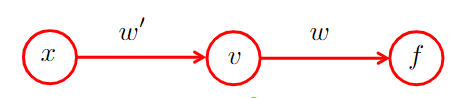
\includegraphics[width=.5\textwidth]{figures/simple_ann_differentiation_example.png}
    \caption{The computation graph of a simple ANN}
    \label{simple_ann_differentiation_example}
\end{figure}

For a slightly more complex example, as depicted in figure \ref{aan-loss-more-complex-example}, the loss is defined as follows:

\begin{equation*}
    L = \sum_{i=1}^{2}\ell_i(\sum_{j}w_{i,j} \varphi(\sum_{k}w'_{j,k} x_k)).
\end{equation*}

The weight vector $\mathbf{W}$ is defined as $\mathbf{W} = [(w_{i,j})_{i,j},(w'_{i,j})_{i,j}]$. The loss is then defined as:

\begin{align*}
    \frac{\partial L}{\partial w_{i,j}}&=\frac{\partial L}{\partial f_{i}}\frac{\partial f_{i}}{\partial w_{i,j}}=\ell'_i(f_i)\cdot v_j\\
\end{align*}

Note that $\ell'_i(f_i)$ and $\cdot v_j$ are computed using forward propagation.

\begin{equation*}
    \frac{\partial L}{\partial w'_{j,k}}=\sum_{i=1}^{2}\frac{\partial L}{\partial f_{i}}\frac{\partial f_i}{\partial v_j}\frac{\partial v_j}{\partial w'_{j,k}}=\sum_{i=1}^{2}\delta_i w_{i,j}\cdot\phi'(z_j)\cdot x_k
\end{equation*}

where $\delta_i=\frac{\partial L}{\partial f_{i}}$ and $\delta '_j=\delta_i w_{i,j}\cdot\phi'(z_j)\cdot x_k$

\begin{figure}
    \centering
    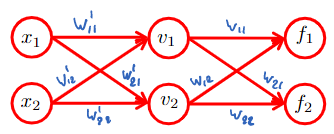
\includegraphics[width=.5\textwidth]{figures/aan-loss-more-complex-example.png}
    \caption{A more complex neural network.}
    \label{aan-loss-more-complex-example}
\end{figure}

\subsubsection{Derivatives of activation functions}

Sigmoid: 
\begin{equation*}
    \varphi(z)=\frac{1}{1+\exp(-z)}
\end{equation*}

\begin{equation*}
    \phi'(z)=\frac{-1}{(1+\exp(-z))^2}\cdot e^{-z}\cdot (-1)=\frac{e^{-z}}{1+e^{-z}}\cdot\frac{1}{1+e^{-z}}=\phi(z)(1-\phi(z))
\end{equation*}

The advantage of this function is that it is differentiable everywhere, however $\phi(z)\approx 0$ unless $z=\approx 0$. This leads to a problem that is called a vanishing gradient for deep models. 

Rectified linear unit (ReLU):
\begin{equation*}
    \varphi(z)=\max(z,0)
\end{equation*}

\begin{equation*}
    \varphi'(z)=\begin{cases}
        1 \text{ if }z>0\\
        0 \text{ otherwise}
    \end{cases}
\end{equation*}

The disadvantage of this function is that it is not differentiable at 0, but in practice this is not a problem. A huge advantage is $\varphi'(z)=1$ for all $z>0$ which helps with avoiding vanishing gradients.

\subsection{Backpropagation}
The unvectorized version of the backpropagation algorithm is as follows:
\begin{enumerate}
    \item For each unit $j$ on the output layer
    \begin{itemize}
        \item Compute the error signal $\delta_j=\ell_j'(f_j)$
        \item For each unit $i$ on layer $L$, compute $\frac{\partial}{\partial w_{i,j}}=\delta_jv_i$
    \end{itemize}
    \item For each unit $j$ on hidden layer $\ell=L-1:-1:1$
    \begin{itemize}
        \item Compute the error signal: $\delta_j=\phi'(z_j)\sum_{i\in\text{Layer}_{\ell+1}}w_{i,j}\delta_i$
        \item For each unit i on layer $\ell$, compute $\frac{\partial}{\partial w_{i,k}}=\delta_{j}v_i$
    \end{itemize}
\end{enumerate}

The vectorized implementation of the backpropagation algorithm can be phrased as follows:
\begin{enumerate}
    \item For the output layer
    \begin{itemize}
        \item Compute the error $\delta^{L}=\mathbf{\ell'(f)}=[\ell'(f_!),\dots, \ell'(f_p)]$
        \item Gradient: $\nabla_{\mathbf{W}^{(L)}}\ell(\mathbf{W};\mathbf{y},\mathbf{x})=\delta^{(L)}\mathbf{v}^{(L-1)T}$
    \end{itemize}
    \item For each hidden layer $\ell=L-1:-1:1$
    \begin{itemize}
        \item Compute the error $\delta^{(\ell)}=\varphi'(\mathbf{z}^{(\ell)})\odot(\mathbf{W}^{(\ell +1) T}\delta^{(\ell+1)})$: 
        \item Compute the gradient: $\nabla_{\mathbf{W}^{(\ell)}}\ell(\mathbf{W};\mathbf{y},\mathbf{x})=\delta^{(\ell)}\mathbf{v}^{(\ell-1)T}$
    \end{itemize}
\end{enumerate}

\subsection{Initializing weights}

Because the optimization problem is non-convex, the initialization of the weights matters, i.e. if we pick innapropriate weights we are more likely to converge towards a suboptimal point in the optimization landscape. Random initialization is often preferred. The rationale of this comes from the propagation of variance. In order to understand why this is the case, assume a node $v_i^{(\ell)}$ with inputs $v_1^{(\ell -1)},\ldots,v_{n_{in}}^{(\ell -1)}$. We know that we carry out the computation $z_i^{(\ell)}=\sum_{j=1}^{n_{in}}w_{ij}v_j^{(\ell-1)}\Rightarrow v_i^{(\ell)}=\phi(z_i^{(\ell)})$ where $\phi(z)=\max(0,z)$. 

\subsubsection{Variance propagation}

Now, we assume $\mathbb{E}[x_i]=\mathbb{E}[v_i^{(0)}]=0$ where $v_i^{(0)}$ is the input layer and we also assume that $\text{Var}[x_i]=\text{Var}[v_i^{(0)}]=1$. Let us further assume that the $X_1, \ldots, X_d$ are independent. Additionally, we assume that the weights are draw from a normal distribution, i.e. $w_{ij}\sim\mathcal{N}(0,1)$. Finally, we know that, supposing $X,Y$ are independent with $\mathbb{E}[X]=0$:
\begin{enumerate}[a]
    \item if $\mathbb{E}[Y]=0$, then $\text{Var}(X,Y)=\text{Var}(X)\text{Var}(Y)$
    \item if $\mathbb{E}[Y]\neq 0$, then $\text{Var}(X,Y)=\text{Var}(X)\mathbb{E}[Y^2]$
    \item For ReLU and symmetric $Y$: $\mathbb{E}[\phi(Y)^2]=\frac{1}{2}\text{Var}(Y)$
\end{enumerate}

We then compute:

\begin{align*}
    \mathbb{E}[z_i^{(1)}]&=\mathbb{E}\left[\sum_{j=1}^{n_{in}} w_{i,j}x_j\right]=\sum_{j}\mathbb{E}[w_{ij}]\mathbb{E}[x_j]=0\\
    \text{Var}[z_i^{(1)}]&=\sum_{j}\text{Var}[w_{ij}x_j]\myeq\sum_{j}\text{Var}(w_{ij})\sum_{j}\text{Var}(x_{j})=n\cdot \sigma^{2}\\
    \text{Var}[z_i^{(1)}]&=\sum_{j}\text{Var}\left[w_{ij}v_j^{(\ell - 1)}\right] = \sum_{j}\text{Var}(w_{ij})\mathbb{E}\left[v_j^{(\ell -1)2}\right]=\frac{1}{2}n_{\text{in}}\sigma^2\coloneqq 1\Rightarrow\sigma^2=\frac{2}{n_{\text{in}}}      
\end{align*}

This means that in this setting (of course heavily idealized), that the random variables will have the same scale with the same variance across each layer.

\subsubsection{Weight initialization strategies}

The goal of any weight initialization procedure is to keep the variance of weights approximately constant across layers to avoid vanishing and exploding gradients. Usually, random initialization works well, for instance:
\begin{itemize}
    \item Glorot initialization using tanh:
    \begin{align*}
        w_{i,j} &\sim\mathcal{N} (0,1/(n_{in}))\\
        w_{i,j} &\sim\mathcal{N} (0,1/(n_{in}+n_{out}))\\
    \end{align*}
    \item He (ReLU):
    \begin{equation*}
        w_{i,j}\sim\mathcal{N}(0,2/n_{in})
    \end{equation*}
\end{itemize}

The effect of improper initialization strategies is that the weights do not converge over time, as shown in figure \ref{weight-init-he-xavier}.

\begin{figure}
    \centering
    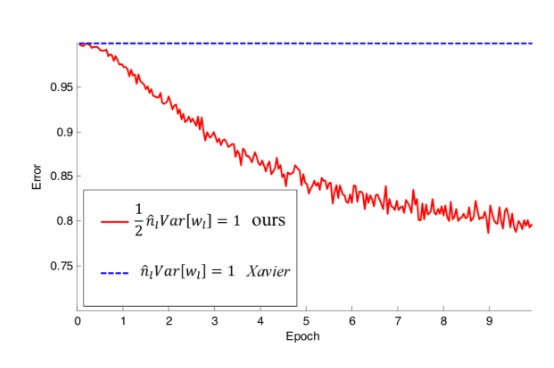
\includegraphics[]{figures/weight-init-he-xavier.png}
    \caption{Weight initialization procedure and effect on training}
    \label{weight-init-he-xavier}
\end{figure}

\subsection{Learning rate}

To implement the SGD rule, a learning rate needs to be chosen. Usually, its a good idea to start with a fixed small learing rate, and decrease slowly after some iteration, e.g.:
\begin{equation*}
    \eta_t=\min (0.1, 100/t)
\end{equation*}
Often, a piecewise constant learning rate schedules the drop in learning rate, e.g. drop after some number of epochs.

Learning with momentum is a common extension to training with SGD as it can help to escale local minima. The idea behind this approach is to not only move into the direction of the gradient, but also in direction of the last weight update. In this case the weight update looks like this:

\begin{align*}
    a&\leftarrow m\cdot a+\eta_t\nabla\ell(\mathbf{W};\mathbf{y},\mathbf{x})
    \mathbf{W}&\leftarrow\mathbf{W}-a
\end{align*}

This allows getting over flatter surfaces of the optimization function quicker while also avoiding oscillations towards the end of the optimization process as we near the optimal point, see figure \ref{oscillation-momentum}. 

\begin{figure}
    \centering
    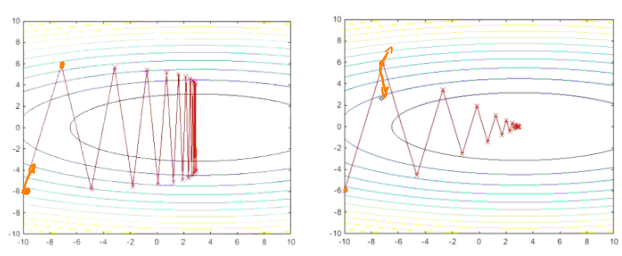
\includegraphics[width=.8\textwidth]{figures/oscillation-momentum.png}
    \caption{Oscillations of the optimization function.}
    \label{oscillation-momentum}
\end{figure}

\subsection{Weight-space symmetries}\label{weight-space-symmetries}

Multiple distinct weights compute the same prediction. I.e. given a network of the topology provided in figure \ref{weight-space-symmetries-fig}, and we define the following variables:
\begin{align*}
    v_i &= \phi(\mathbf{w}_i,x)\\
    f &= w_1'v_1+w_2'v_2\\
    \mathbf{w}=[w_i,w_i']_i&,\bar{\mathbf{w}}=[\bar{w_i},\bar{w_i'}]_i
\end{align*} 

Suppose $\bar{\mathbf{w}_2}=\mathbf{{w}}_1$, $\bar{\mathbf{w}_1}=\mathbf{{w}}_2$, $\bar{\mathbf{w}_1'}=\mathbf{{w}}_2'$, $\bar{\mathbf{w}_2'}=\mathbf{{w}}_1'$, we then have:
\begin{equation*}
    f(\mathbf{x};\bar{\mathbf{w}})=f(\mathbf{x};\mathbf{w})
\end{equation*}
which means that multiple local minima can be equivalent in terms of input-output mapping.

For instance, this is valid for the tanh activation function, where $\varphi(z)=-\varphi(-z)$

\begin{figure}
    \centering
    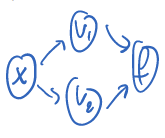
\includegraphics[]{figures/weight-symmetries.png}
    \caption{Network topology used to illustrate weight-space symmetries shown in section \ref{weight-space-symmetries}.}
    \label{weight-space-symmetries-fig}
\end{figure}

\subsection{Avoiding overfitting}

Due to the fact that neural networks have multiple parameters, they have the potential of overfitting the data. There are several countermeasures that can be adopted to mitigate this phenomenon:
\begin{itemize}
    \item Early stopping: it consists in stopping SGD until it converges. This is done by monitoring the prediction performance on a validation set and stop trainign once the validation error starts to increase. 
    \item Regularization: add penalty term to keep the weights small. 
    \begin{equation*}
        \hat{\mathbf{W}}=\arg\min_{\mathbf{W}}\sum_{i=1}^{n}\ell(\mathbf{W};\mathbf{x}_i,y_i)+\lambda\norm{W}_{F}^2
    \end{equation*}
    \item Dropout: the key idea here is to randomly ignore hidden units during each iteration of SGD with probability $p$. At test time, we then multiply the weights by the probability $p$.
    \item Batch normalization: inputs are shifted and scaled through each layer. Batch normalization is a widely used technique that normalizes inputs to each layer according to mini-batch statistics.
    \begin{itemize}
        \item It reduces internal covariate shift
        \item Enables larger learning rates
        \item It helps with regularization.
    \end{itemize}
\end{itemize}

The algorithm for batch normalization goes as follows:
\begin{enumerate}
    \item \textbf{Input}: values of $x$ over a mini-batch: $\mathcal{B}=\left\{x_1,\ldots,m\right\}$; Parameters to be learned: $\gamma,\beta$
    \item \textbf{Output}: $\left\{y_i=\textnormal{BN}_{\gamma,\beta}(x_i)\right\}$
    \begin{align*}
        \mu_{\mathcal{B}}&\leftarrow\frac{1}{n}\sum_{i=1}^{m}x_i &\text{mini-batch mean}\\
        \sigma_{\mathcal{B}}^2&\leftarrow\frac{1}{n}\sum_{i=1}^{m}(x_i-\mu_{\mathcal{B}})^2&\text{mini-batch variance}\\
        \hat{x_i}&\leftarrow \frac{x_i-\mu_{\mathcal{B}}}{\sqrt{\sigma_{\mathcal{B}}^2+\epsilon}}&\text{normalize}\\
        y_i&\leftarrow \gamma\hat{x}_i+\beta\equiv\text{BN}_{\gamma, \beta}(x_i)&\text{scale and shift}
    \end{align*}
\end{enumerate}
After this procedure, $\phi(\mathbf{w}\mathbf{x})\rightarrow\phi(\mathbf{w}\textnormal{B}_{\gamma,\beta}(\mathbf{x}))$

\subsection{Invariances}
Predictions should be unchanged under some transformations of the data, e.g.
\begin{itemize}
    \item Classification of handwritten digits: the digit can be anywhere on the picture 
    \item Speech recognition: the pitch should not matter for classification the speed of the speech should also not matter.
\end{itemize} 
A model can be encouraged to learn specific invariances via the following methods:
\begin{itemize}
    \item Augmentation of the training set
    \item Special regularization terms
    \item Invariance built into pre-processing
    \item Implement invariance into structure of ANN, e.g. using convolutional neural networks.
\end{itemize}

\subsection{Convolutional neural networks}
Convolutional neural networks are ANNs for specialized applications, e.g. for image recognition. The hidden layers closest to the input layer shares parameters: each hidden unit only depends on all closeby inputs, e.g. pixels and weights contrained to be identical across all units on the layer. This reduces the number of parameters, and encourages robustness against small amounts of translation. The weights can still be optimized using backpropagation.

The typical CNN architecture that we see is that similar to the one shown in figure \ref{cnn-arch}.

\begin{figure}
    \centering
    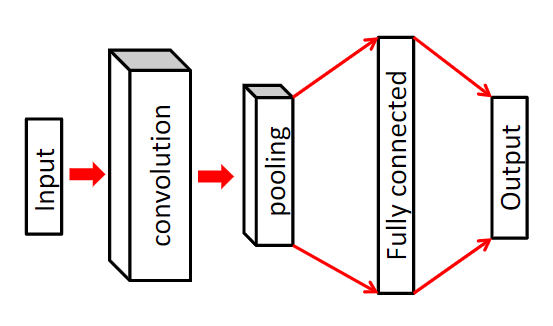
\includegraphics[width=.5\textwidth]{figures/cnn-arch.png}
    \caption{Typical architecture of a CNN}
    \label{cnn-arch}
\end{figure}

Important aspects of CNN have specific terminologies:
\begin{itemize}
    \item Filters/kernels: the size of the filter that passes over an image
    \item Stride: the size of the step taken by the filter at each iteration
    \item Padding: the distance between the border of the image and the first pixel to be processed. 
\end{itemize}

Computing the output dimensions of a CNN can be done as follows. Applying $m$ different $f\times f$ filtes to an $n\times n$ image with padding $p$ and stride $s$, we get an output measurement of $\ell=\frac{n+2p-f}{s}+1$. In some applications (e.g. image classification), it can make sense to aggregate several units to decrease the width of the network (and hence the number of parameters). 

Pooling layers (equivalent to subsampling) can be added. In some applications, e.g. in image classification, it can make sense to aggregat several units to decrease the width of the network and hence the number of parameters. Usually, one considers either the average or the maximum value of the resulting output of the filter, see figure \ref{max-pooling-layers}.

\begin{figure}
    \centering
    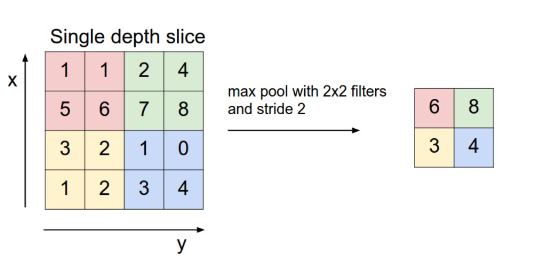
\includegraphics[width=.5\textwidth]{figures/max-pooling-layers.png}
    \caption{Max pooling layers example.}
    \label{max-pooling-layers}
\end{figure}

An example of CNN architecture can be found in figure \ref{cnn-arch}.

\begin{figure}
    \centering
    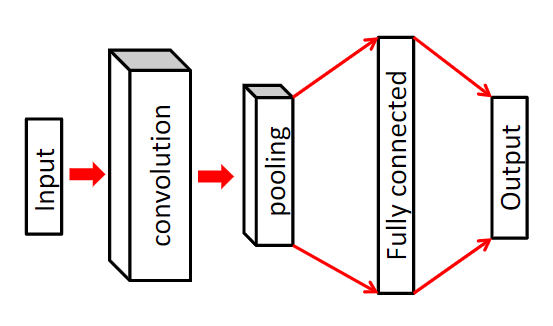
\includegraphics[width=.5\textwidth]{figures/cnn-arch.png}
    \caption{Typical CNN architecture.}
    \label{cnn-arch}
\end{figure}

\subsection{Computational efficiency}

A key operation for backpropagation training is the dense matrix vector multiplications. These are very suitable on general purpose GPUs and much work on special purpose hardware, for instance TPUs. They have been reponsible for large improvement in computations in recent years. 

\subsection{Choice of parameters and architectures}

Several possible activation functions are available. Popular in the past were sigmoid and tanh activations, because they were differentiable. Recently, however, rectified linear units (ReLUs) have been used. Despite being not differentiable, they are very fast to compute and gradients do not vanish, which is important for deep neural networks.

A number of parameters have to be chosen:
\begin{itemize}
    \item The number and width of hidden layers 
    \item Use convolution/pooling layers and how many
    \item Skip connections
    \item Type of activation functions
    \item Weight initialization
    \item Learning rate schedule
    \item Regularization method
\end{itemize}

Frameworks for autodifferentiation, e.g. theano, torch and tensorflow. They can use cross-validation to compare models, but training is usually very expensive. They often use single validation (=development) set. Much work is also being done on ML-based experimentaion, i.e. AutoML.

\subsection{ANNs vs. kernels}

When using the tanh activation function, an ANN with a single hidden layer learns functions of the form:
\begin{equation*}
    f(\mathbf{x})=\sum_{i}w_i\tanh\theta^{T}_i\mathbf{x}
\end{equation*}
This is exactly the same type of functions learned with kernels, when using the tanh kernel.
\begin{equation*}
    f(\mathbf{x})=\sum_{i}\alpha_i\tanh\mathbf{x}_i^T\mathbf{x}
\end{equation*}
The difference is that kernels optimize $\alpha$'s only. It is therefore convex. ANNs, however, optimize both $\mathbf{w}'s$ and $\theta_i$, which is a non-convex problem. A more comprehensive comparison of ANNs and kernels is summerized in table \ref{kernels-vs-anns}.

\begin{table}
    \centering
    \begin{tabulary}{\textwidth}{Lp{170pt}p{170pt}}
        \toprule
        \textbf{Method} & \textit{Method} & \textit{ANNs}\\
        \midrule
        \textbf{Advantages} & Convex optimization, no local minima, robust against noise, models grow with the size of the data & Flexible nonlinear models, with fixed parametrization. Multiple layers discover representations at multiple levels of abstraction\\
        \textbf{Disadvantages} & Models grow with the size of data, don't allow multiple layers. & Many free parameters/architectural choices that need to be tuned. Often suffer from very noisy data.  \\
    \end{tabulary}
    \label{kernels-vs-anns}
\end{table}

\end{document}